% !TeX encoding = UTF-8
% !TeX spellcheck = en_US
% !BIB TS-program = biber
% basic packages and document settings
\documentclass[a4paper,12pt]{article}
\usepackage[english]{babel}
\usepackage[utf8]{inputenc}
\usepackage[T1]{fontenc}
\usepackage[a4paper]{geometry}
\geometry{top = 30mm, bottom = 25mm, left = 25mm, right = 25mm}
\usepackage{setspace}
\onehalfspacing
\raggedbottom
\pdfcompresslevel9

% mathmode-related packages
\usepackage{mathtools}
\usepackage{physics}
\usepackage{amsmath}
\usepackage{amsthm}
\usepackage{amsbsy}
\usepackage{mathrsfs}
\usepackage{amssymb}
\usepackage{amstext}
\usepackage{amsfonts}
\usepackage{tikz}
\usepackage{siunitx}
%\usepackage{IEEEtrantools}

% misc
\usepackage{esdiff}
\usepackage{multirow}
\usepackage{blindtext}
\usepackage{todonotes}
\usepackage{abstract}
\usepackage{appendix}
\usepackage[bottom]{footmisc}
\usepackage{listings}
\usepackage{dashrule}

% graphics and floats
\usepackage{graphicx}
\graphicspath{{../Figures/}}
\usepackage{tikz}
\usepackage{float}
\usepackage{wrapfig}
%\usepackage{subfloat}
\usepackage{subcaption}
%\usepackage{caption}
\usepackage[rightcaption]{sidecap}
\usepackage{tabularx}
\usepackage{adjustbox}
%\usepackage{svg}
\usepackage{epstopdf}
\usepackage{grffile}	% handle file names with dots, spaces etc.
%\usepackage{flafter}
\usepackage{rotating}
%\usepackage{floatrow}
%\floatsetup[figure]{capposition=beside,capbesideposition={top,right}}

%\usepackage{epstopdf}
%\epstopdfDeclareGraphicsRule{.pdf}{png}{.png}{convert #1 \OutputFile}
%\AppendGraphicsExtensions{.pdf}

% packages requiring setup arguments

\usepackage{xcolor}
%\definecolor{rwth-dark}{HTML}{176daf}
\definecolor{rwth-dark}{RGB}{0,84,159}
%\definecolor{rwth-light}{HTML}{8abae3}
\definecolor{rwth-light}{RGB}{142,186,229}

%/**
%* Generated by Gpick 0.2.5
%* RWTH Dark: #176daf, rgb(23, 109, 175), hsl(32, 43%, 69%)
%* RWTH Light: #8abae3, rgb(138, 186, 227), hsl(195, 73%, 89%)
%*/

\usepackage{hyperref}
\hypersetup{hidelinks=true,colorlinks=true,allcolors=rwth-dark}
\usepackage[nameinlink,capitalise]{cleveref}
%\usepackage[hyphens]{url}
%\urlstyle{sf}
%\usepackage{breakurl}


% header & footer settings
\usepackage{fancyhdr}
\pagestyle{fancy}
%\renewcommand{\chaptermark}[1]{\markboth{#1}{}} % with this we ensure that the chapter and section headings are in lowercase.
\renewcommand{\sectionmark}[1]{\markright{\thesection\ #1}}
\fancyhf{} % delete current header and footer

%\fancyhead[LE,RO]{\large\thepage}
\fancyhead[L]{\large\rightmark}
\fancyhead[R]{\large\leftmark}

\renewcommand{\headrulewidth}{0.3pt}
\renewcommand{\footrulewidth}{0pt}
%\addtolength{\headheight}{0.5pt} % space for the rule

\fancyfoot[C]{\thepage}

\fancypagestyle{plain}
{
	\fancyhead{} % get rid of headers on plain pages
	\renewcommand{\headrulewidth}{0pt} % and the line
}

% ========== command definitions =================================
\newcommand{\Thickline}{\rule{\linewidth}{0.4mm}}
\newcommand{\Thinline}{\rule{\linewidth}{0.1mm}}

\newcommand{\id}{\, \mathrm{d}}

\definecolor{codegray}{gray}{0.9}
\newcommand{\code}[1]{\colorbox{codegray}{\texttt{#1}}}

\newcommand{\skippage}{\clearpage{\thispagestyle{empty}\cleardoublepage}}

\def\@esphack{%
	\relax
	\ifhmode
	\spacefactor\@savsf
	\ifdim\@savsk>\z@
	\ignorespaces
	\fi
	\fi}

\title{\LARGE title}
\date{}


\begin{document}
	
\begin{titlepage}
	\thispagestyle{empty}
	\newgeometry{top=20mm, left=20mm, right=20mm, bottom=20mm}
	
%	\begin{minipage}{0.35\textwidth}
%		\begin{flushleft}
%
%
%		\end{flushleft}
%	\end{minipage}
%	\hfill
%	\begin{minipage}{0.65\textwidth}
%		\begin{flushright}
%
%		\end{flushright}
%	\end{minipage}
	
%	\vspace*{\fill}
	\hspace{0pt}
	\vspace{2cm}
	\begin{center}
%		\Thickline
%		\vskip -0.5cm
%		\Thinline
		\hdashrule{\linewidth}{2pt}{}
		\vskip -0.5cm
		\hdashrule{\linewidth}{1pt}{}
		
		\vspace{0.5cm}
		\Huge{ \textbf{ T2 \\}}
		\LARGE{ \textbf{Gamma spectroscopy and Compton scattering } } 
		
		\hdashrule{\linewidth}{1pt}{}
		\vskip -0.9cm
		\hdashrule{\linewidth}{2pt}{}
%		\Thinline
%		\vskip -0.9cm
%		\Thickline 
		
		\vspace{3cm}
		\Large{\textbf{ Group 14 \\}}
		\Large{Alexandre Drouet, 358681 \\ Olexiy Fedorets, 356615 \\}
		\vspace{1cm}
		\Large{\textsl{ Experiment Date: 19.--20.02.2019 \\ Submission Date: 06.03.2019}}

		

		
	\end{center}
	\vfill
%	\vspace*{\fill}
	
\end{titlepage}
	
	
	
\skippage
\pagenumbering{roman}
\thispagestyle{plain}

\tableofcontents
%	\newpage
\listoffigures

\begingroup
\let\cleardoublepage\relax
\let\clearpage\relax
\listoftables
\endgroup
%\listoftables

\skippage

\pagenumbering{arabic}
\setcounter{page}{1}
\restoregeometry
\thispagestyle{fancy}


\skippage
	
\section{Introduction}
In this experiment we want to analyse the Energy of photons emitted by radioactive probes with a szintillaor detector. First we will use Materials with low radiation and with well known energy peaks to calibrate the detector. Then we will use that to analyse the spectrum of a source with stronger radiation and establish a link between scattering angle and the energy of compton scatterd photons. 


\section{Gamma spectroscopy}

\subsection{Theory}
We are looking at photons with energies from 5keV up to 2Mev. There are three relevant interactions of photons with matter within this energy range.\\
Photoelectric effect ($E_\gamma \sim E_B$):\\
Incoming photon with energy Eg is absorbed by an electron with binding energy $E_B$. That electron leaves the Atom with kinetic Energy $E_{\mathrm{kin}} = E_\gamma - E_B$. X-ray radiation follows because of the empty position being filled b an electron of a higher shell.\\
Compton scattering ($E_\gamma \gg E_B$):\\
Incoming Photon is scattered at an electron. It is not absorbed but transmits enrgy to the electron. The maximum transmitted energy is given by $E_C$. That maximum is obtained through frontal collision (scattering angle $\theta = 180^\circ$).\\
Pair production ($E_\gamma \geqslant 2m_ec^2(1+\frac{m_e}{M})$):\\
If the Energy is greater than the mass of two electrons, the photon can decay in a positron and an electron. Given an additional interaction partner with mass $M$ for momentum conservation, a (non-virtual??) positron-electron-pair can be produced. This pair then decays into two photons.\\
\\
The expected energy peaks for an incoming photon with energy $E_\gamma$ are the following:\\
Photo peak at $E_\gamma \leftarrow$ All energy is absorbed.\\
Compton edge at $E_C \leftarrow$ Compton collision with frontal collision and undetected scattered photon.\\
Escape peak at $E_\mathrm{esc}^{(1)} = E_\gamma - m_ec^2 \leftarrow$ Pair production with one undetected final state photon.\\
Double escape peak $E_\mathrm{esc}^{(2)} = E_\gamma - 2m_ec^2 \leftarrow$ Pair production with two undetected final state photon.\\
Backscatter peak $E_R = E_\gamma - E_C \leftarrow$ Compton effect outside of the scintillator with absorption of the scattered photon.\\

\subsection{Setup}

\begin{figure}[H]
	\centering
	\includegraphics[scale=0.1]{../Figures/calib.jpg}
	\caption{Setup for calibration}
	\label{setCalib}
\end{figure}

A radioactive probe is placed in front of the detector at distance $r_0 = (8.7\pm0.1)$cm. The detector is shielded by a collimator with the diameter of the opening being $(2.6\pm0.1)$mm, which gives us a used detector surface of $F_D = (5.3\pm0.4)\si{\centi\meter\squared}$. The detector is placed right behind the collimator to increase intensity and reduce diffraction effects, so that we know the surface of the detector most precisely. We measure the energy spectrum of four different probes, being Cs, Co, Na, Eu. We also do a noise measurement with no probe.

The calculated activities of the radioactive sources used for the experiment are shown in \cref{tab:probes}.
  
\begin{table}[H]
	\renewcommand{\arraystretch}{2}
	\centering
	\large
	\begin{adjustbox}{width=1.1\textwidth}
		\begin{tabular}{|c|c|c|c|c|c|}
			\hline
			& Cs (strong) & Cs (weak) & Co & Eu & Na \\
			\hline
			Buy date & 23.11.2010 & 12.08.1988 & 15.04.2003 & 02.06.1978 & 12.01.2005 \\
			\hline
			Activity at buy date (\si{\kilo\becquerel}) & $44400$ & $37$ & $37$ & $37$ & $37$ \\
			\hline
			Halflife time (days) & $\left(1.100 \pm 0.009\right) \times 10^{4}$ & $\left(1.100 \pm 0.009\right) \times 10^{4}$ & $\left(1.9253 \pm 0.0004\right) \times 10^{3}$ & $\left(4.943 \pm 0.005\right) \times 10^{3}$ & $\left(9.505 \pm 0.004\right) \times 10^{2}$ \\
			\hline
			Decay constant (\si{\per\second}) & $\left(7.29 \pm 0.06\right) \times 10^{-10}$ & $\left(7.29 \pm 0.06\right) \times 10^{-10}$ & $\left(4.1669 \pm 0.0009\right) \times 10^{-9}$ & $\left(1.623 \pm 0.002\right) \times 10^{-9}$ & $\left(8.440 \pm 0.004\right) \times 10^{-9}$ \\
			\hline
			Activity today (\si{\kilo\becquerel}) & $\left(3.673 \pm 0.006\right) \times 10^{4}$ & $\left(1.83 \pm 0.01\right) \times 10^{1}$ & $\left(4.602 \pm 0.002\right) \times 10^{0}$ & $\left(4.60 \pm 0.01\right) \times 10^{0}$ & $\left(8.64 \pm 0.01\right) \times 10^{-1}$ \\
			\hline
		\end{tabular}
	\end{adjustbox}
	\caption{A compilation of all radioactive sources used in the experiment, with corresponding activities computed according to the decay law. }
	\label{tab:probes}
\end{table}


\subsection{Analysis}
Once we substract the noise, we can clearly see the photoeffect peaks we are looking for. We suspect the continuous compton spectrum and the various other peaks to be responsible for what could be described as a source specific noise, increasing in intensity for lower energies.

\begin{figure}[H]
\centering
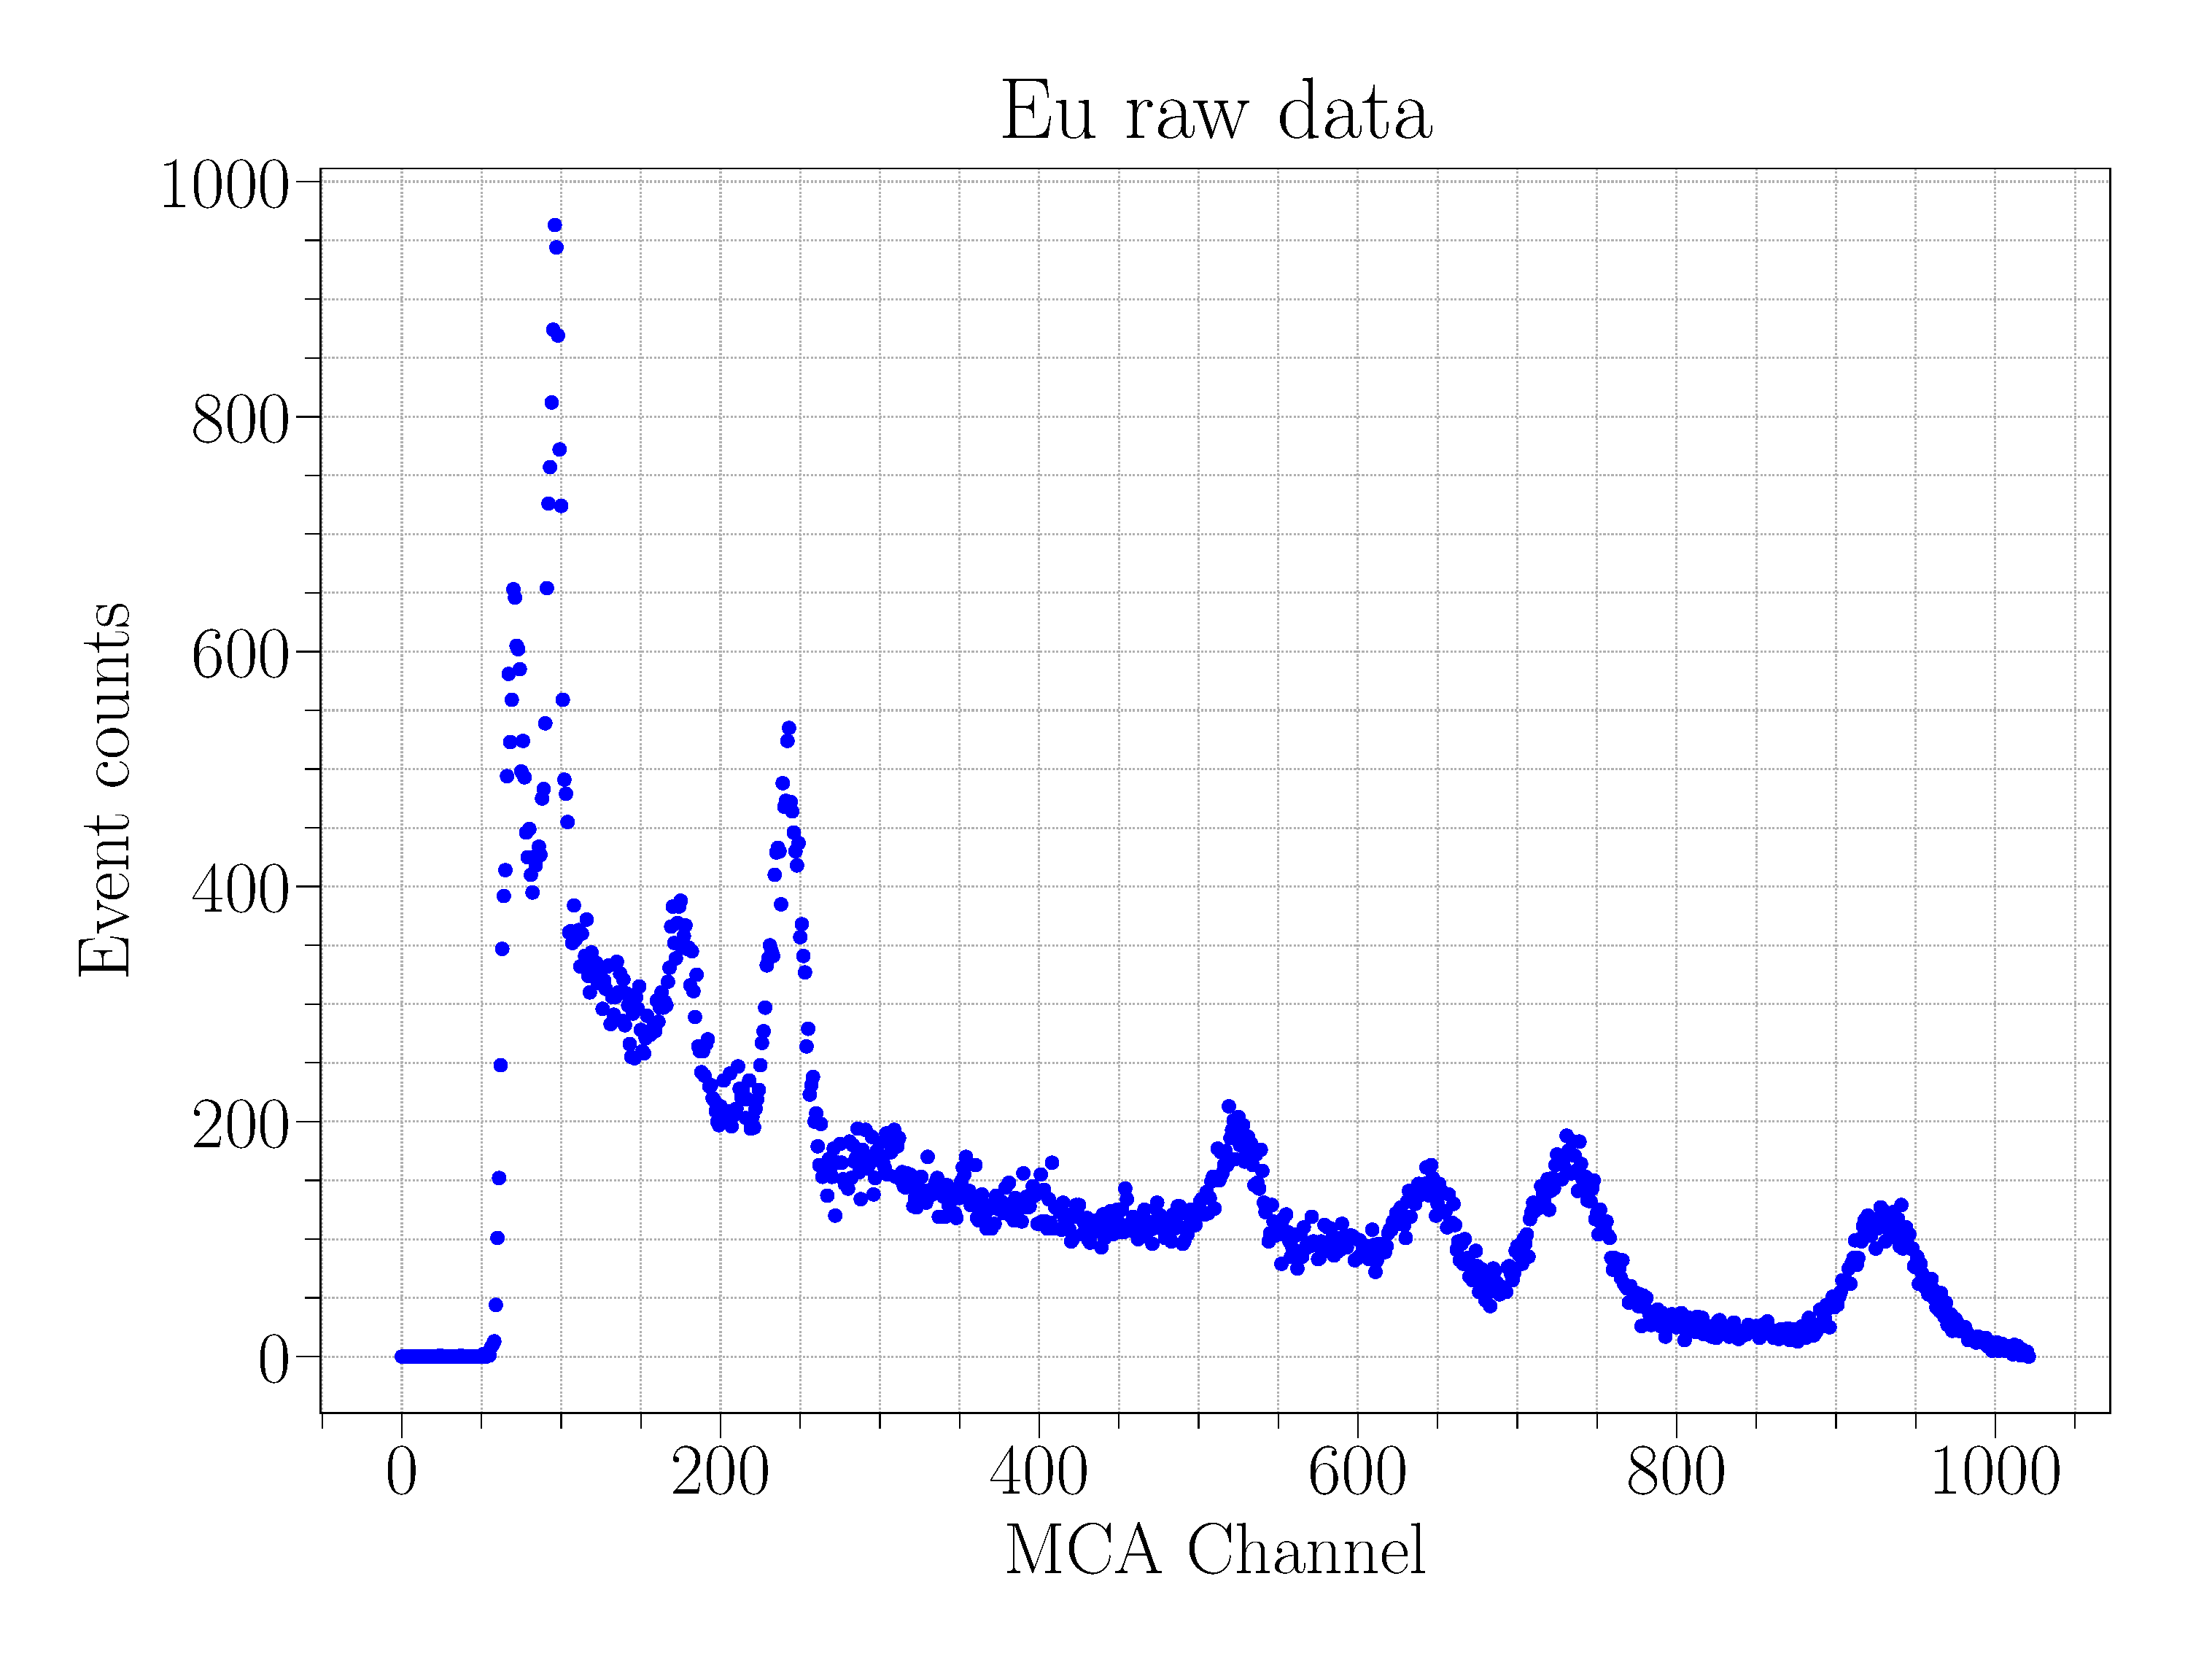
\includegraphics[scale=0.3]{../Figures/Eu_raw.eps}
\caption{Raw data of Eu source}
\label{Eu_raw}
\end{figure}

\begin{figure}[H]
\centering
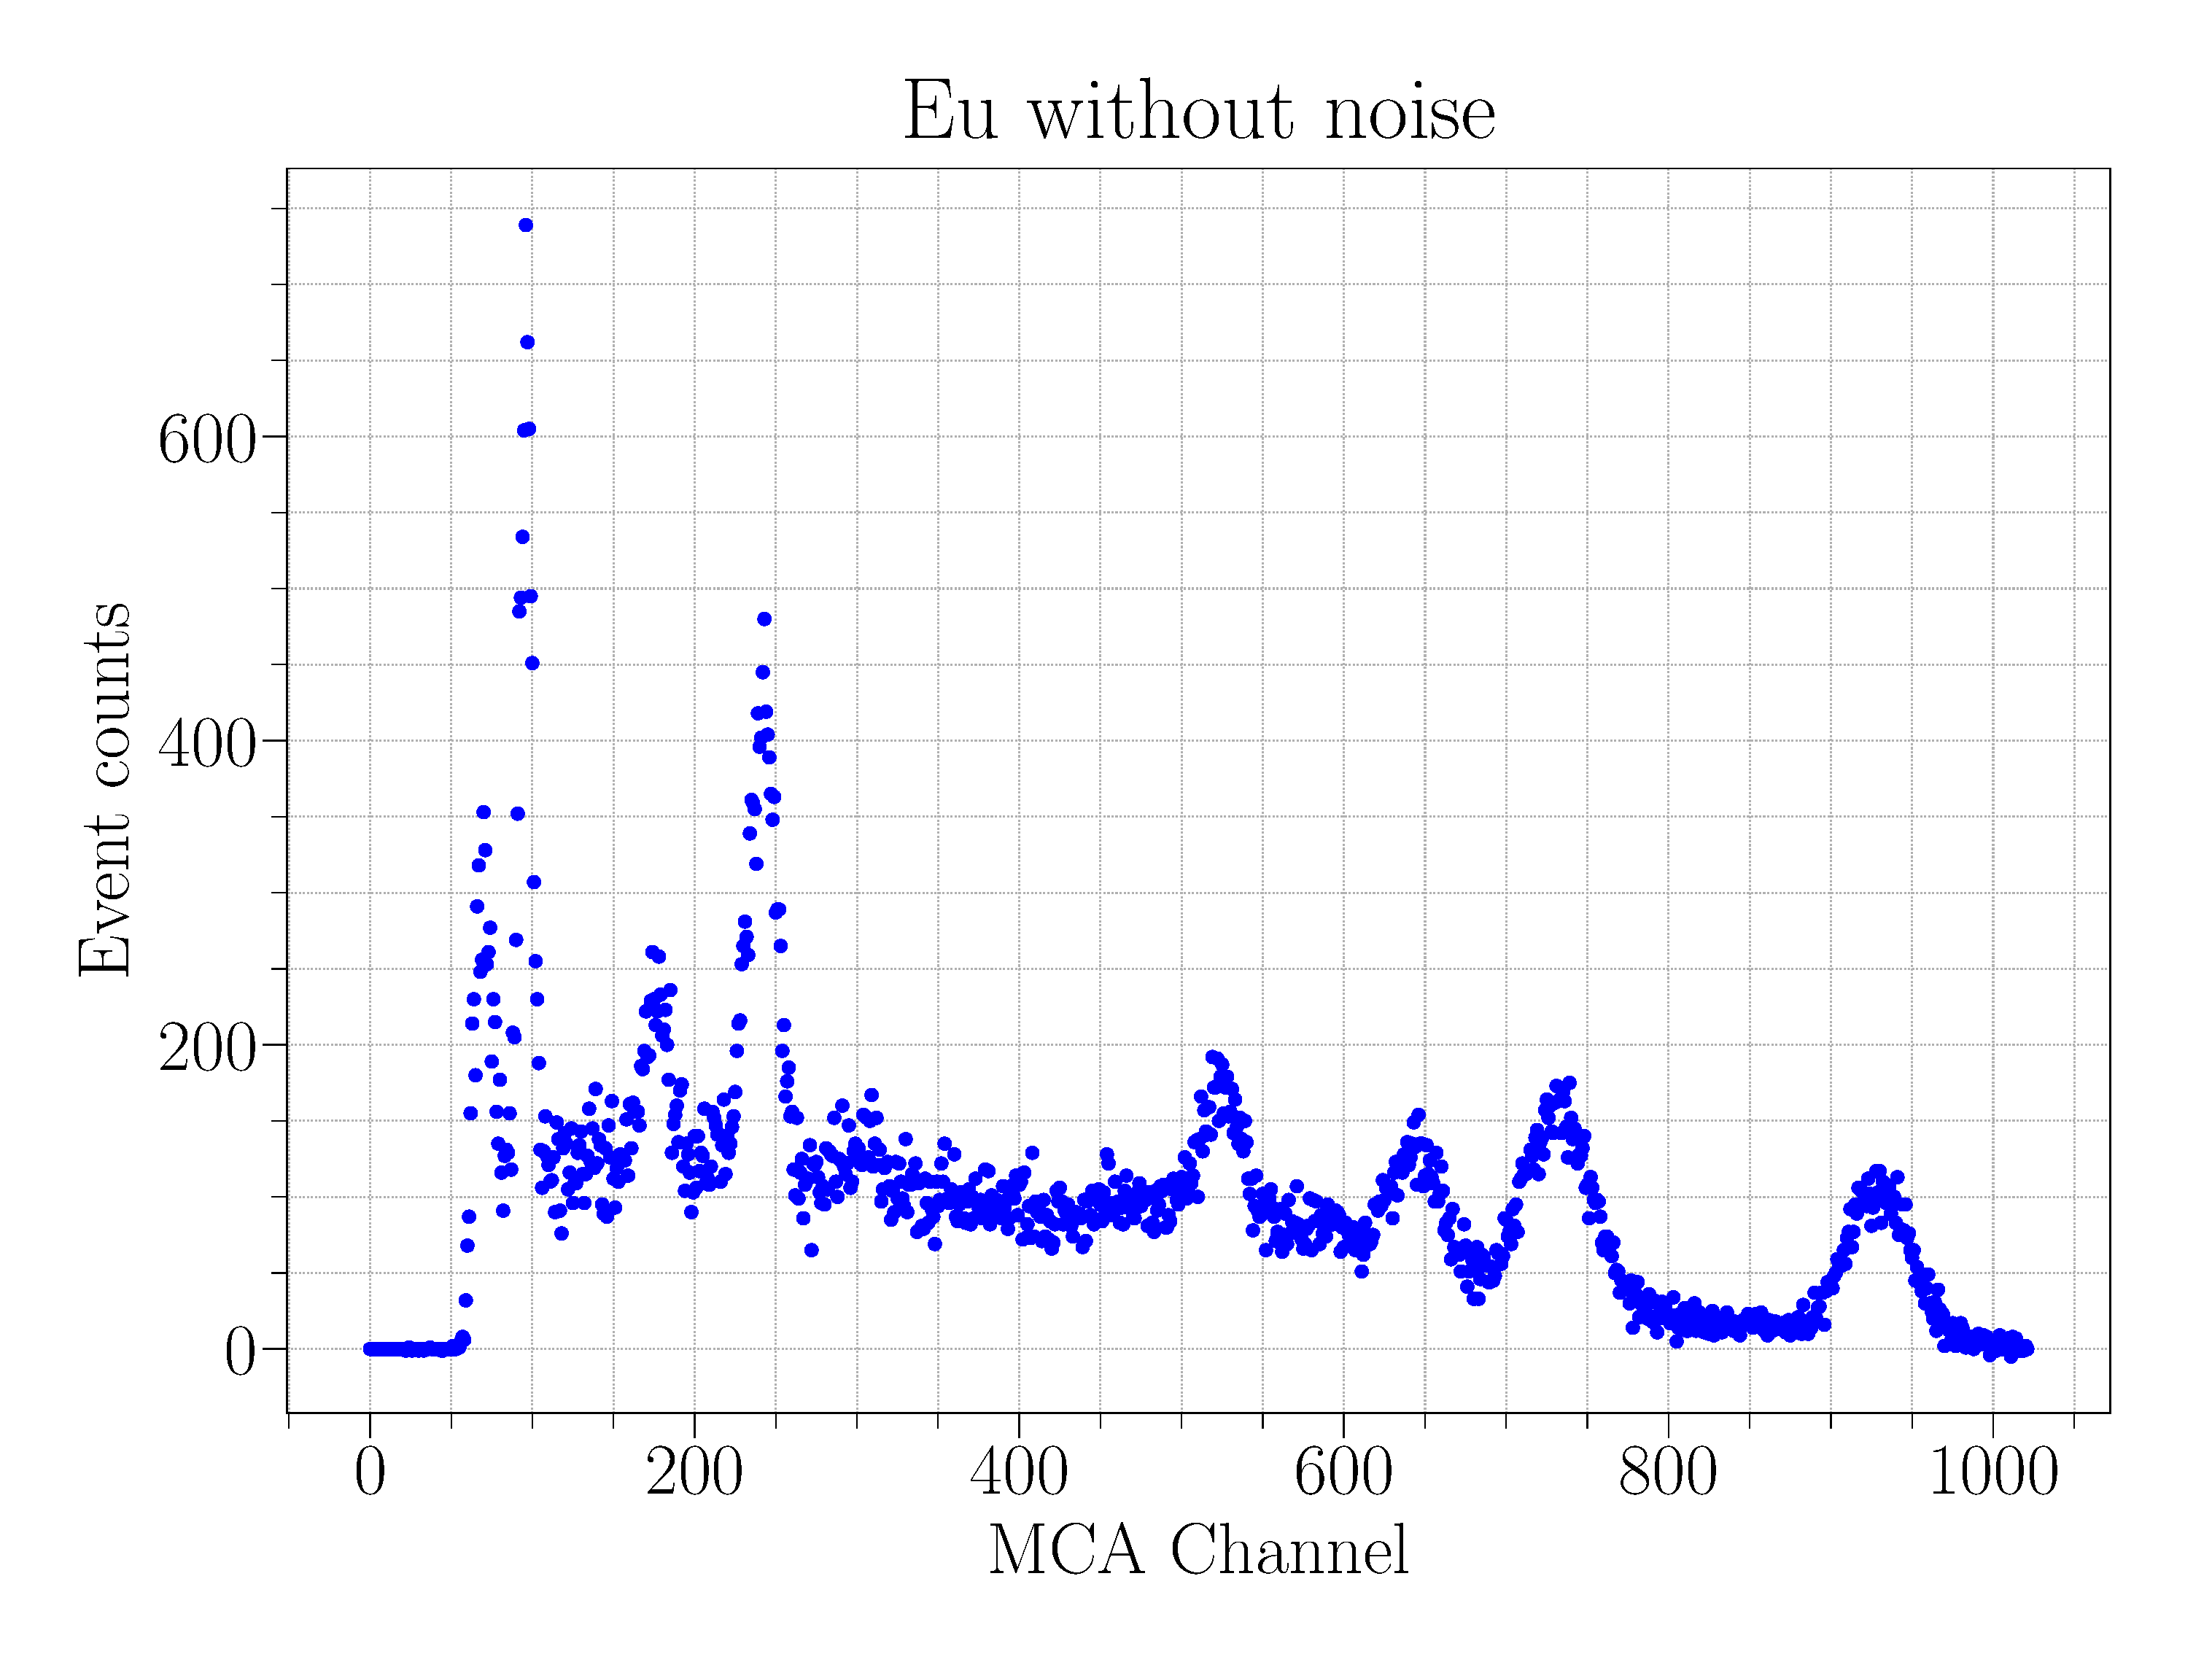
\includegraphics[scale=0.3]{../Figures/Eu_nonoise.eps}
\caption{Eu data after subtraction of noise}
\label{Eu}
\end{figure}

\subsubsection{Calibration}
To find the energies corresponding to channel numbers of the MCA we need to perform a calibration. We fit gaussian curves on the individual peaks in the data and use the center values as calibration points, together with theory values of the peak energies obtained from the datasheets.

An example of this procedure is shown in \cref{Eu_gauss} for Eu. Here we decided to use only the peaks with highest intensities according to the datasheet. We had to leave out one of the large peaks because it produced an outlier in the following analysis. We suspect that multiple energy peaks melded into one because of poor resolution.

To improve the estimate of peak widths, we used a polynomial baseline estimation routine from \code{peakutils.peak.baseline()} to subtract the background level and shift the whole data closer to zero. The resulting datapoints are shown for the example of Eu in \cref{Eu_gauss}.

\begin{figure}[H]
	\centering
	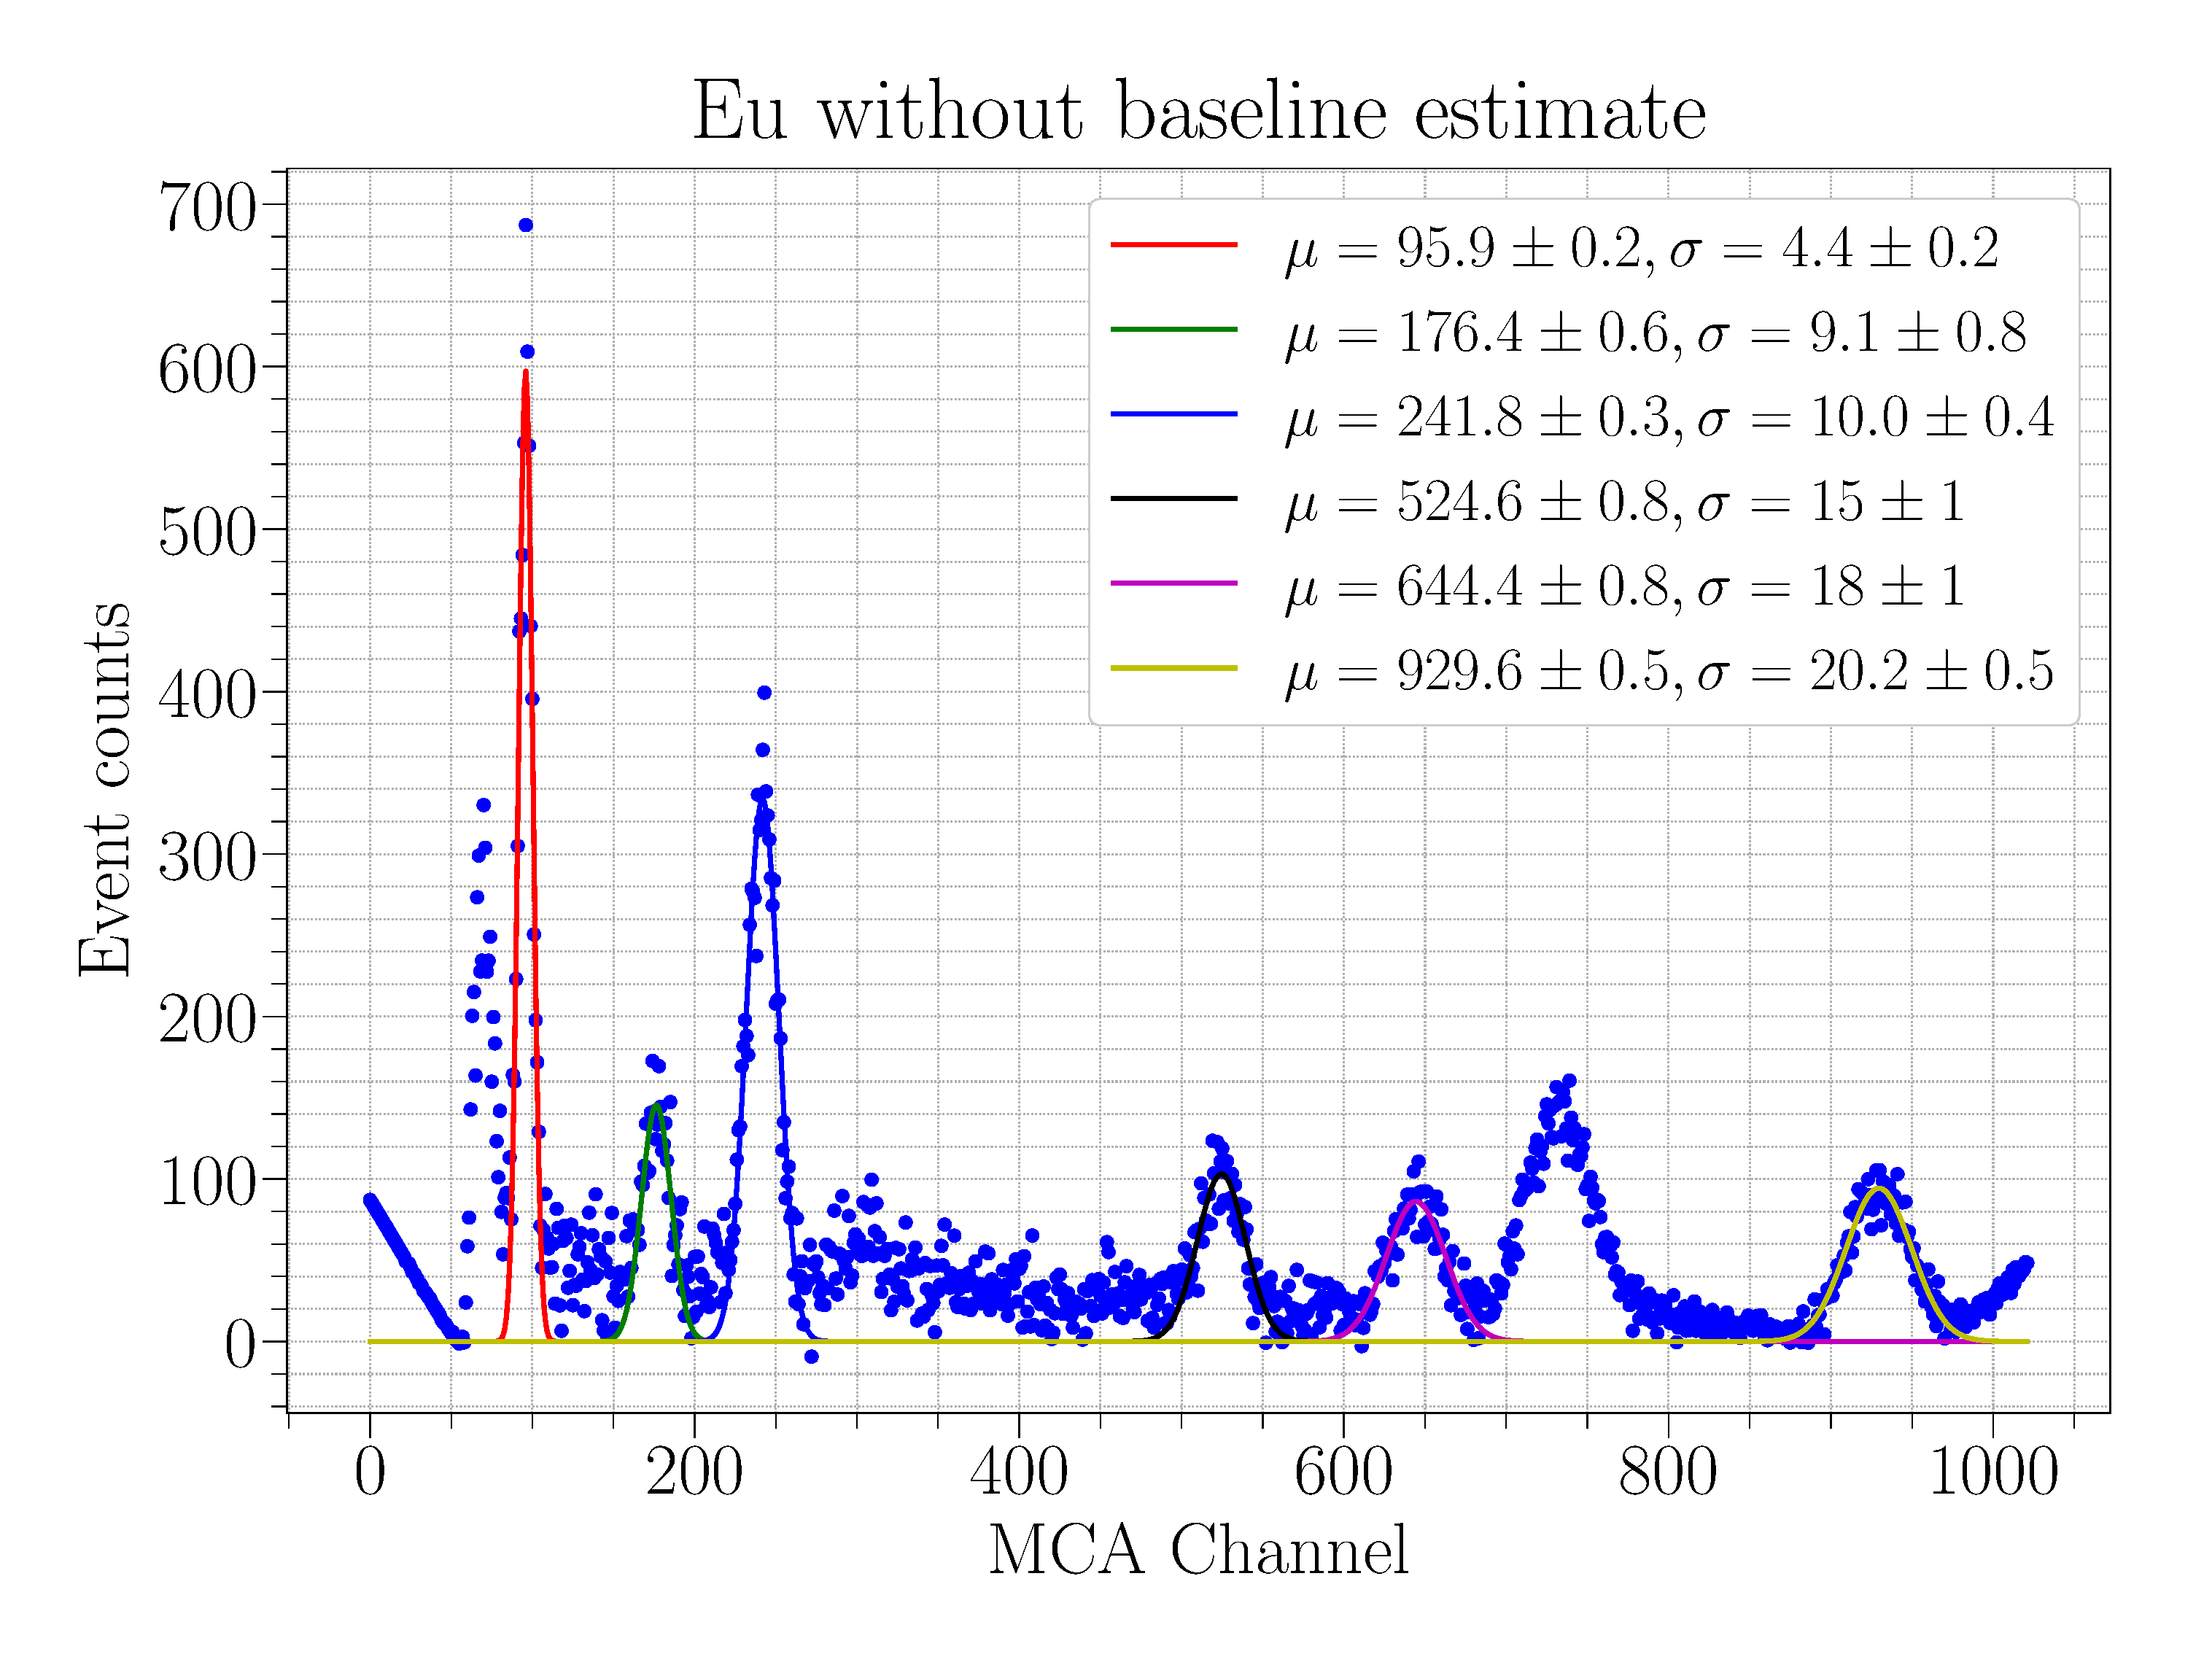
\includegraphics[scale=0.3]{../Figures/Eu_nobaseline.eps}
	\caption{Fitting of gauss peaks in Eu data}
	\label{Eu_gauss}
\end{figure}

Then we proceed to do a linear fit $E_{\gamma} = a \cdot \mathrm{ch}+ b$ with $E_{\gamma}$ being the energies of the peaks we identified, such that we are able to assign an energy to every channel in future evaluations.
The first fit was of poor quality and based on the residuals we decided to split up the fit in two parts for low and high energies, which greatly improved the quality of the respective fits. We thus get two linear regions of our detector.

Complete fit: \newline
$a = 1.544\pm0.003$ \newline
$b = -28.334\pm1.431$ \newline
$\frac{\chi^2}{ndf} = 41.111$ \newline

Fit for lower energies: \newline
$a = 1.533\pm0.001$ \newline
$b = -25.468\pm0.322$ \newline
$\frac{\chi^2}{ndf} = 1.373$ \newline

Fit for higher energies: \newline
$a = 1.553\pm0.007$ \newline
$b = -32.815\pm5.822$ \newline
$\frac{\chi^2}{ndf} = 3.476$ \newline



\begin{figure}[H]
\centering
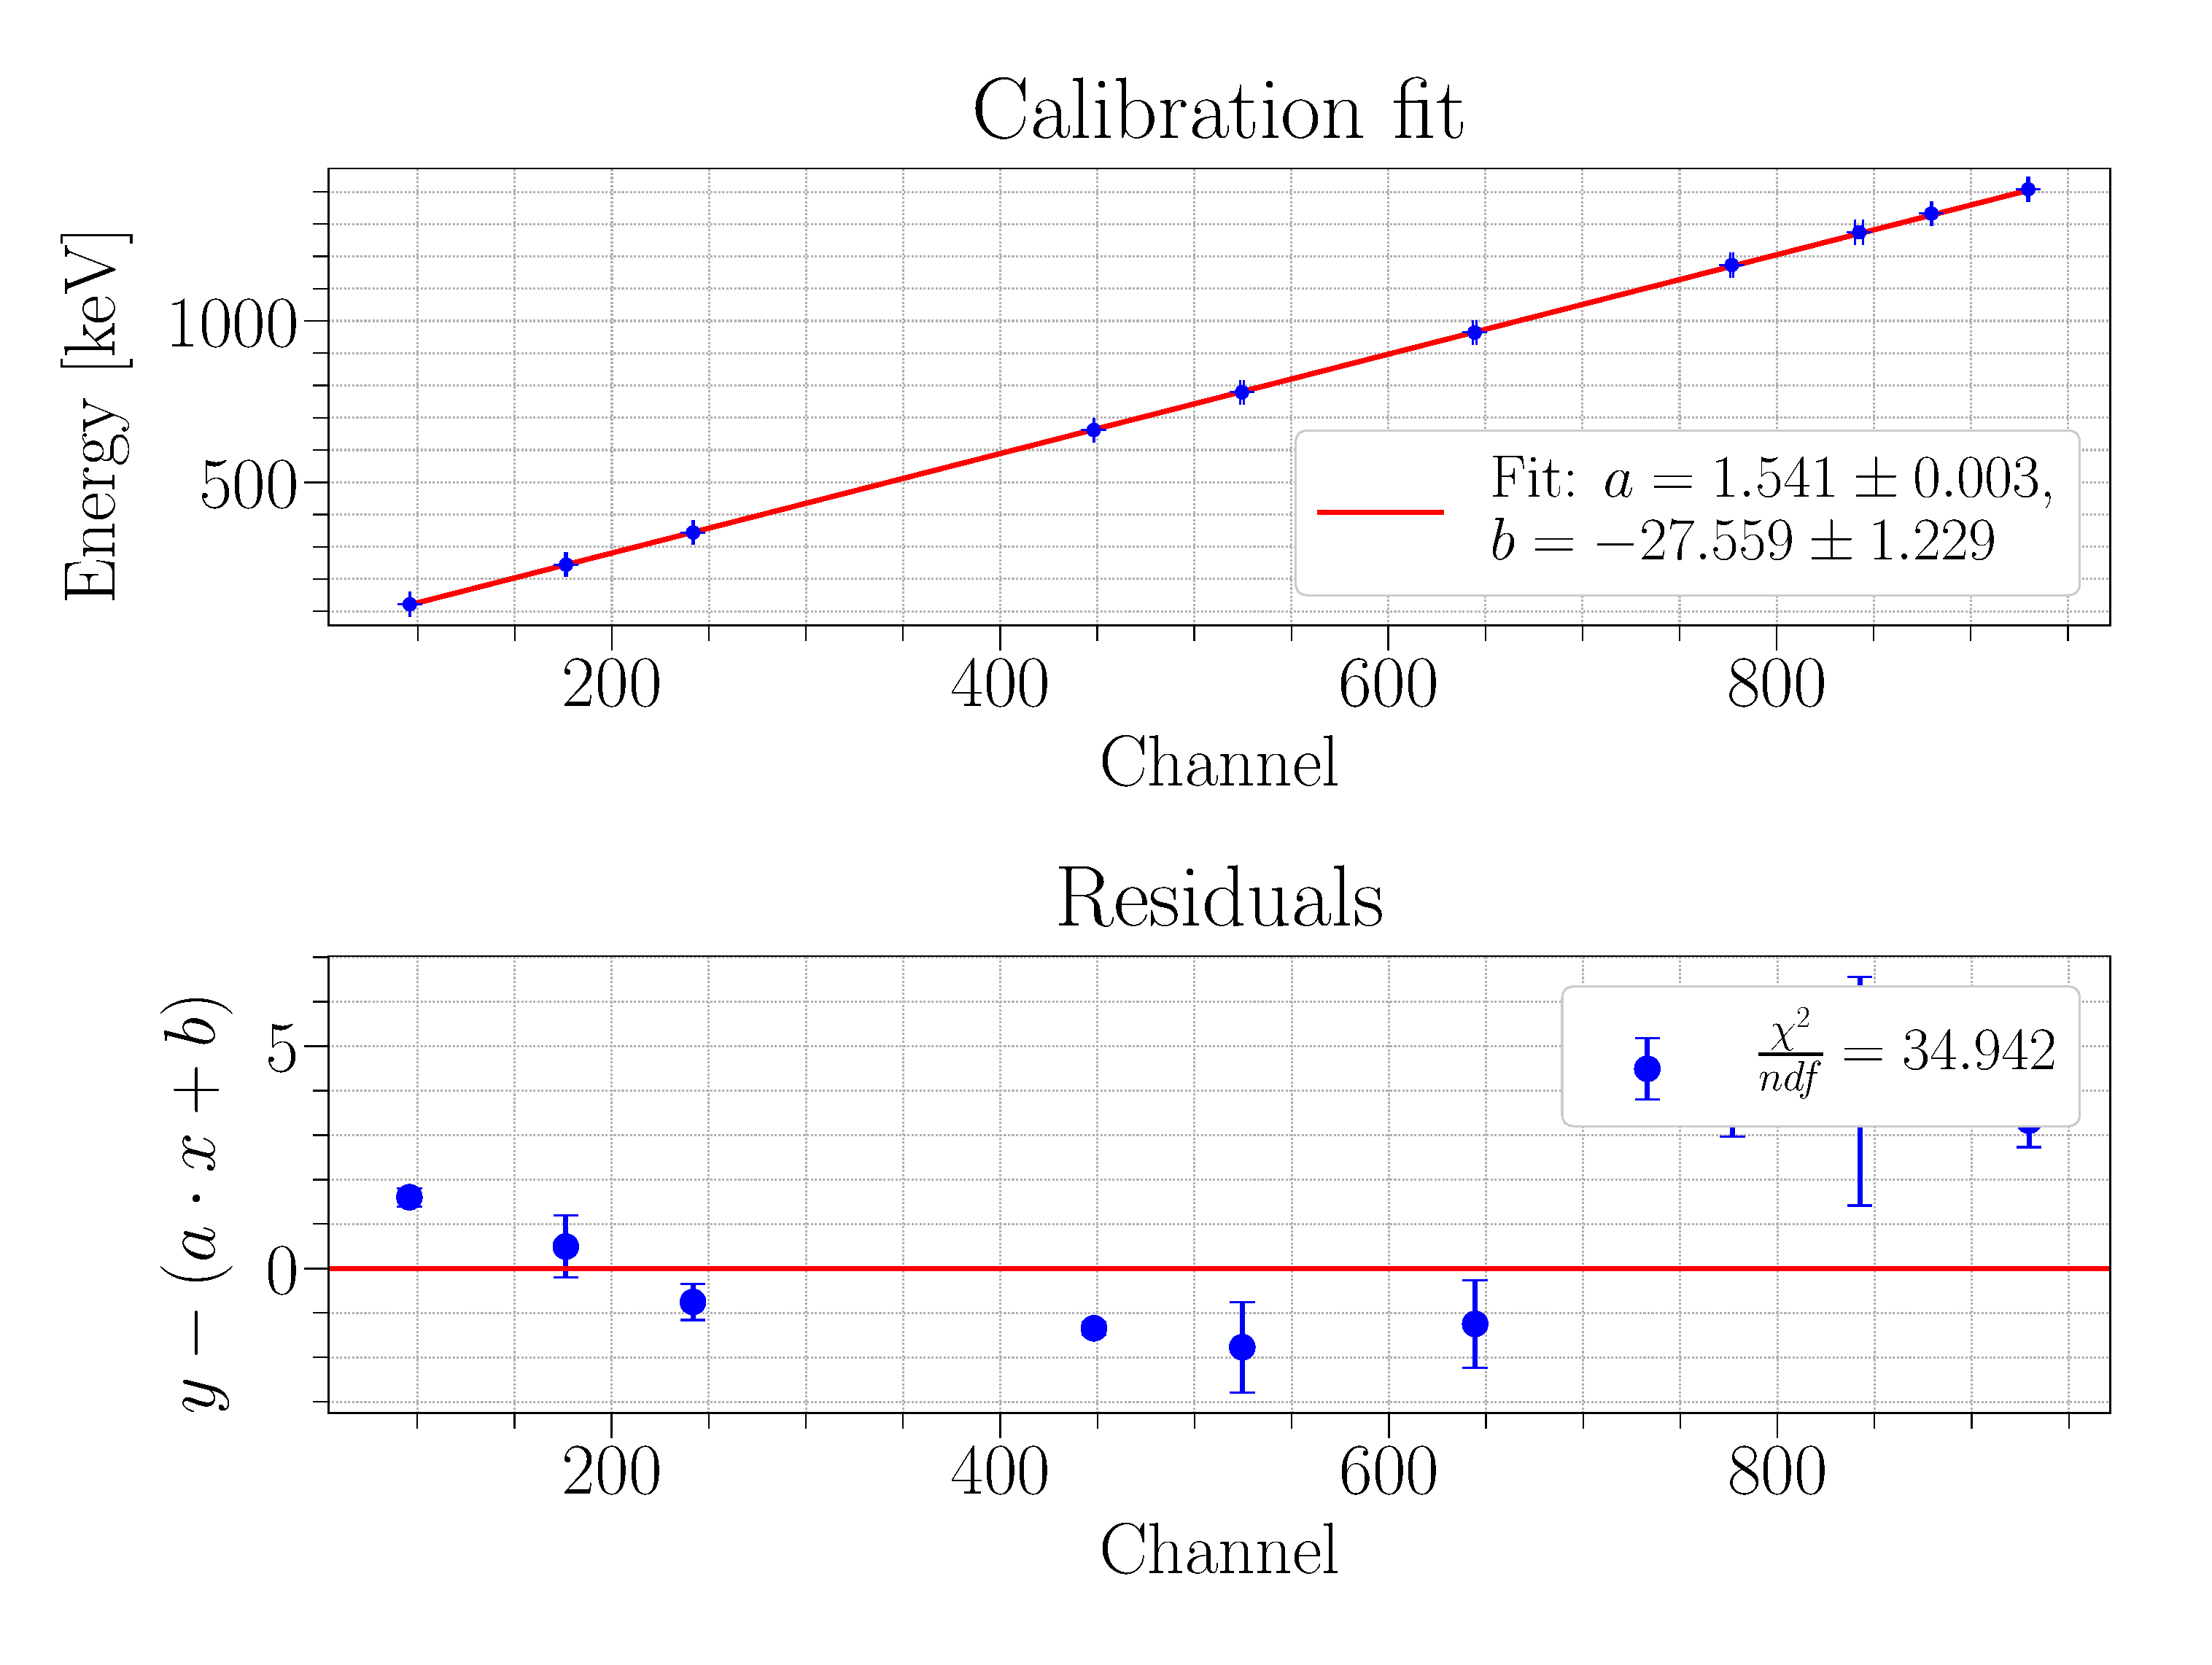
\includegraphics[scale=0.25]{../Figures/Calibration_fit.eps}
\caption{Linear fit for all the energies}
\label{calibFit}
\end{figure}

\begin{figure}[H]
\centering
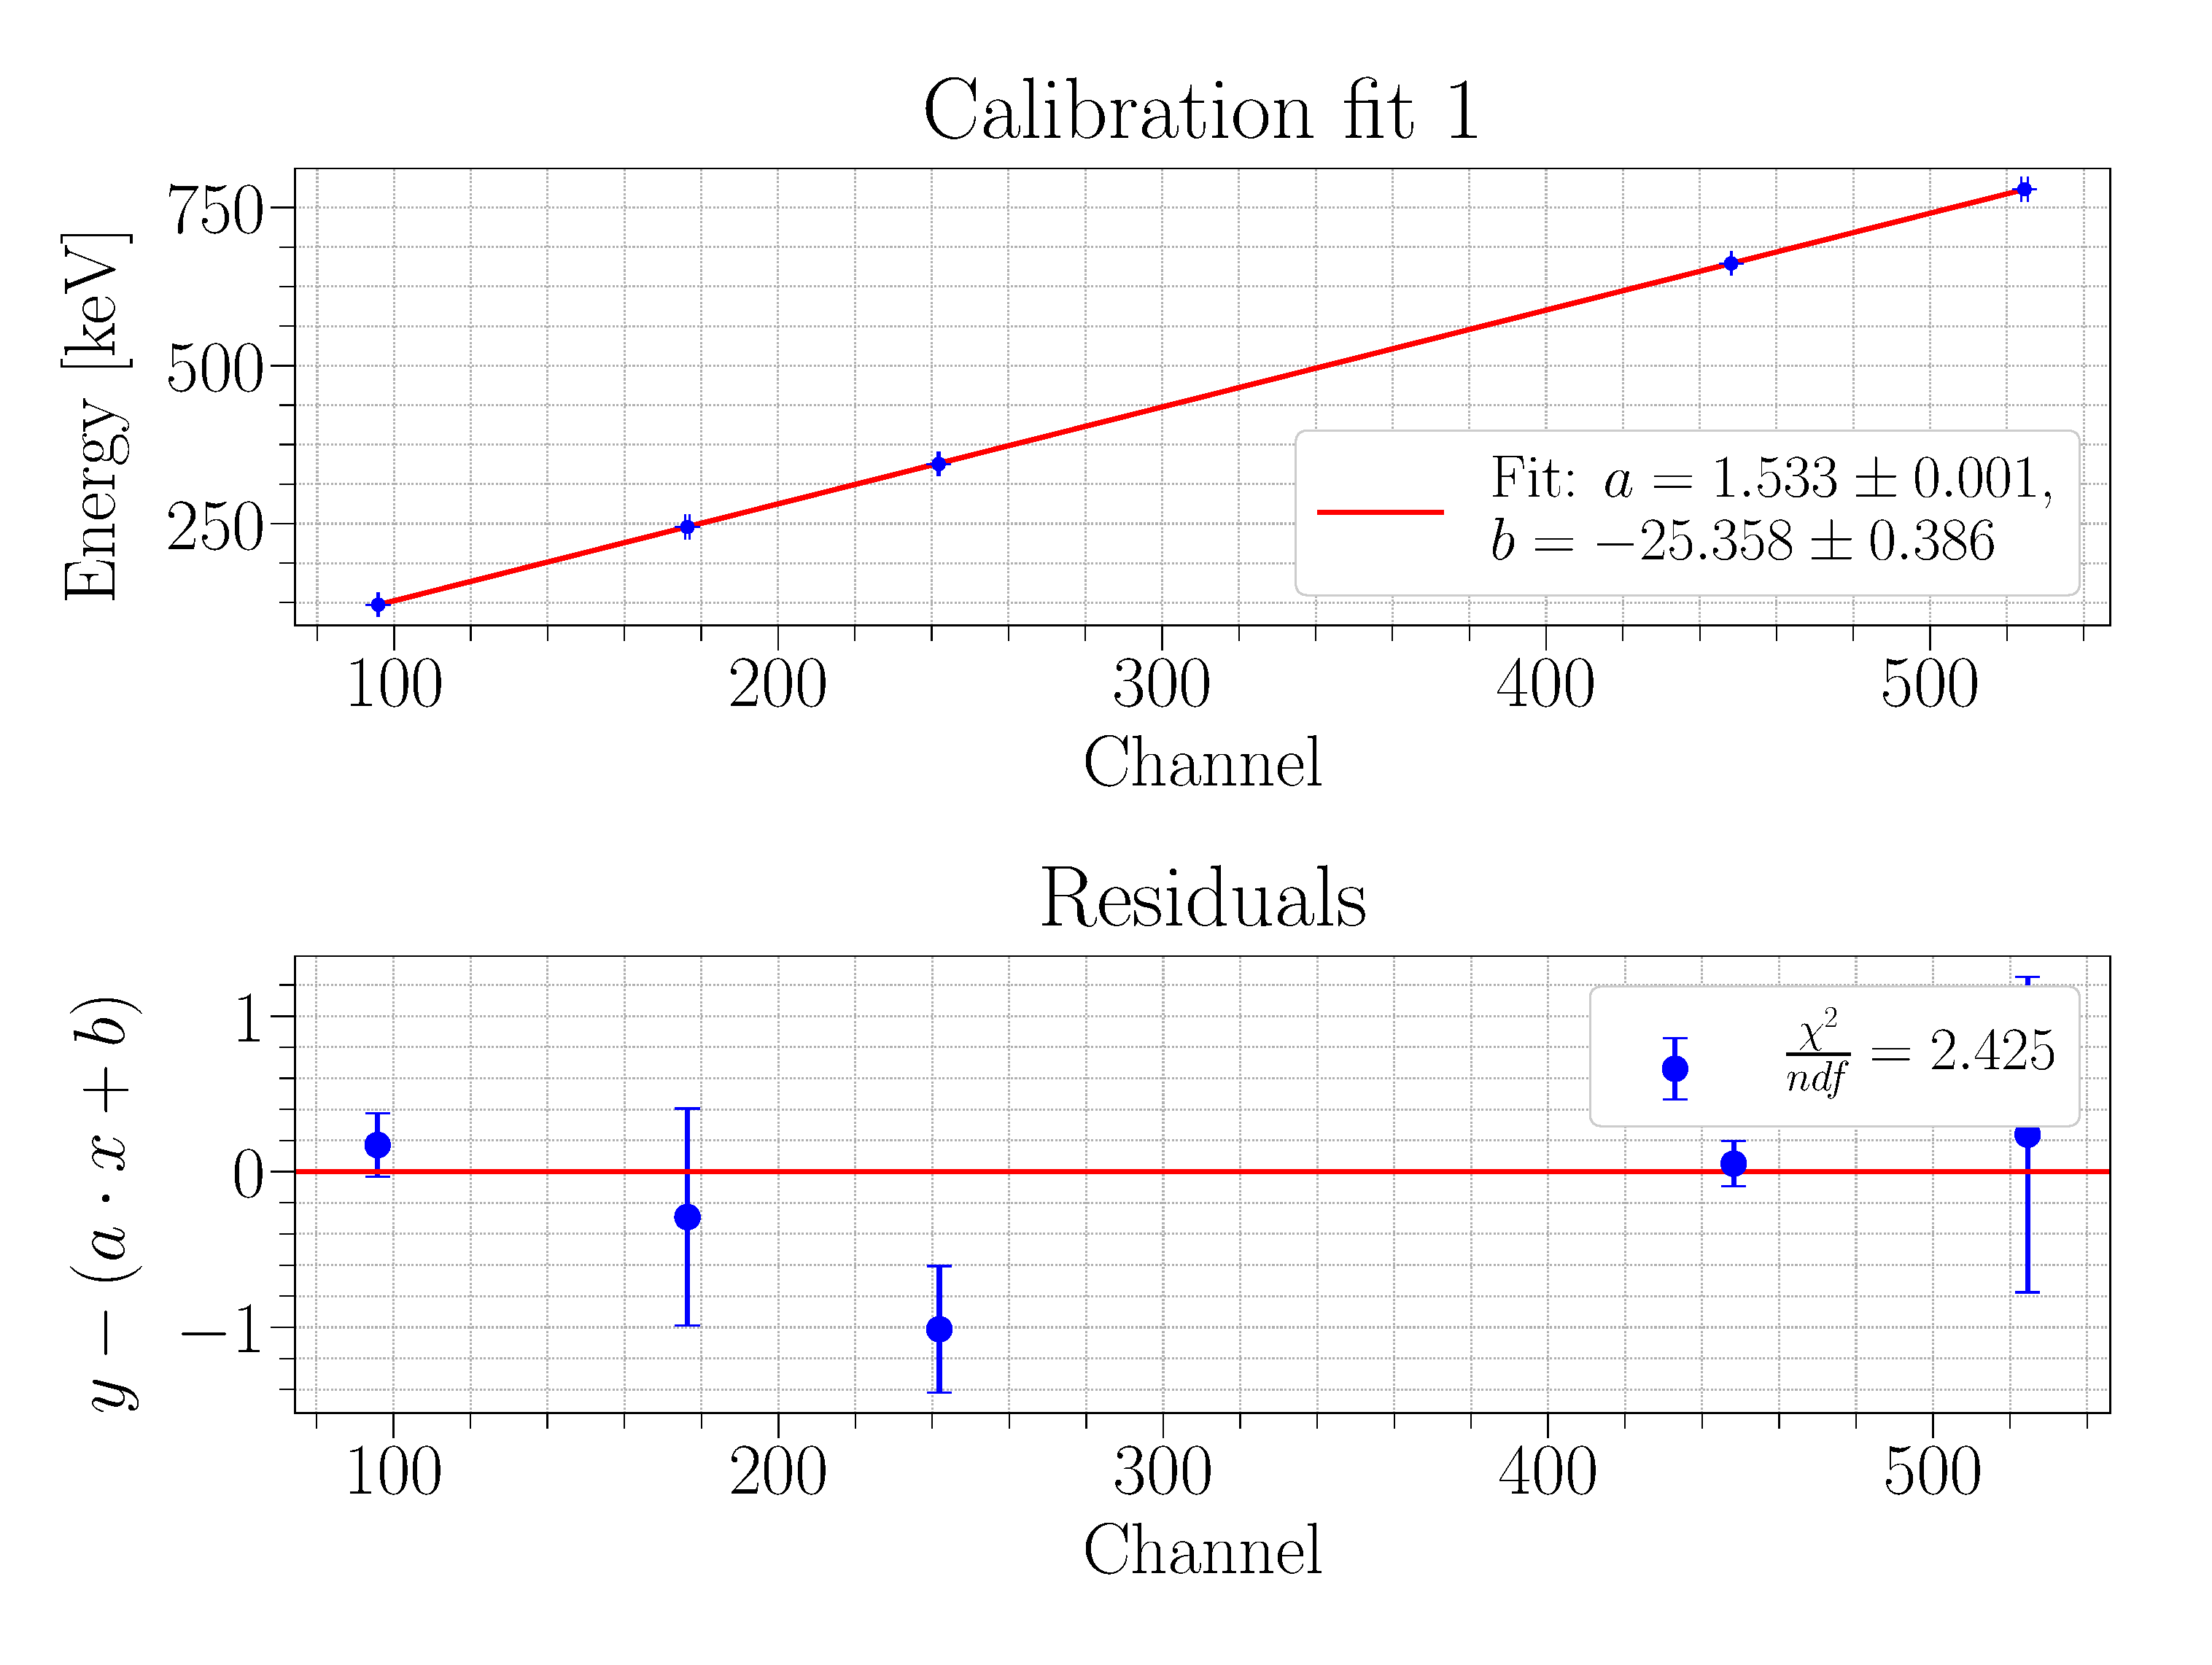
\includegraphics[scale=0.25]{../Figures/Calibration_fit_1.eps}
\caption{Linear fit for lower energies}
\label{calibFit}
\end{figure}

\begin{figure}[H]
\centering
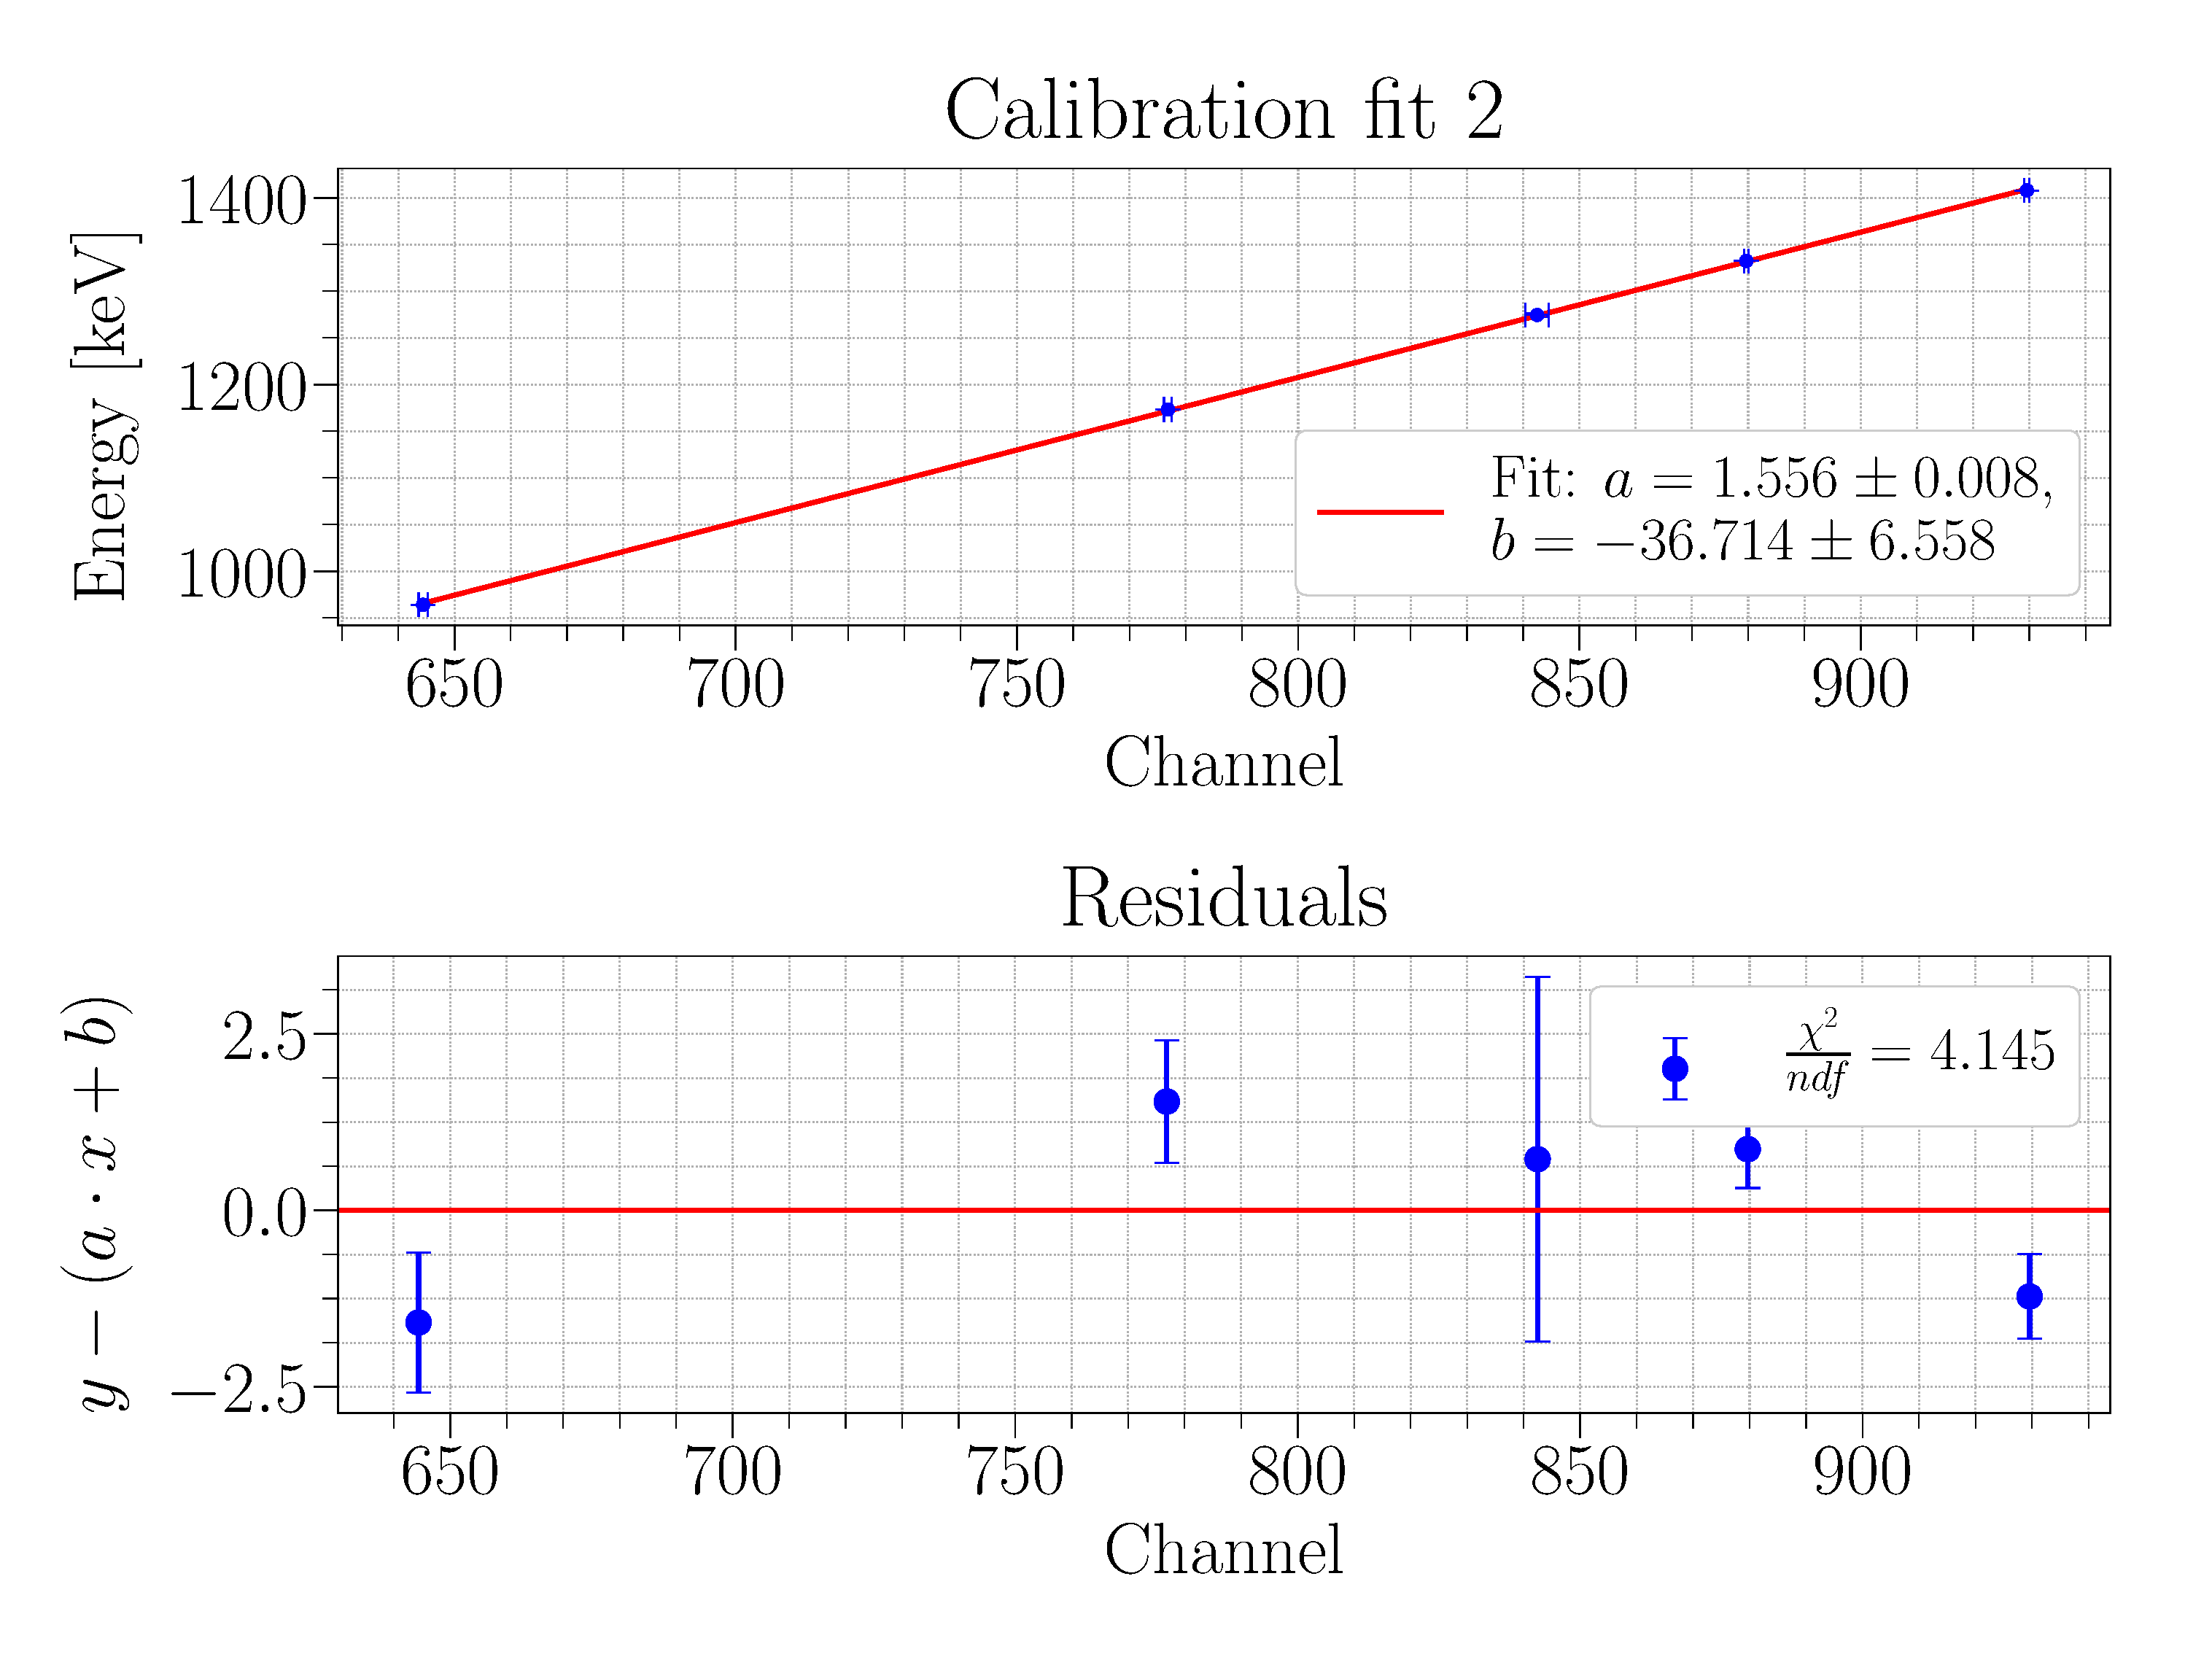
\includegraphics[scale=0.25]{../Figures/Calibration_fit_2.eps}
\caption{Linear fit for higher energies}
\label{calibFit}
\end{figure}

\subsubsection{Energy resolution}
We obtained the resolution by getting the standard deviations of the fitted Gauss curves and converting those to FWHM. Next we calculated the channel values at the FWHM and converted those into energy values based on the previous calibration. Plotting $\Delta E/E$ vs $E$ we see a decline towards higher energies, as it would be expected. Nonetheless we can not see a clear linear dependence.

To find the constants for the systematic contribution $a$ and the statistical contribution (due to Poisson statistics) $b$ in the resolution formula 
\begin{equation}
	\frac{\Delta E}{E} = \sqrt{a^2+ \frac{b^2}{E}}
\end{equation}
we plotted $\Delta E^2$ vs $E$ and fitted the function 
\begin{equation}
	\Delta E^2 = a^2 \cdot E^2 + b^2 \cdot E
\end{equation}

It seems the data does not behave quite as expected, since it doesn't fit well. Nonetheless, the values for $a$ and $b$ we get out of that fit remain our best guess for the resolution constants.
\newline

fit parameters: \newline
$a = 0.032\pm0.009$ \newline
$b = 1.766\pm0.128$ \newline
$\frac{\chi^2}{ndf} = 70.963$ \newline

\begin{figure}[H]
\centering
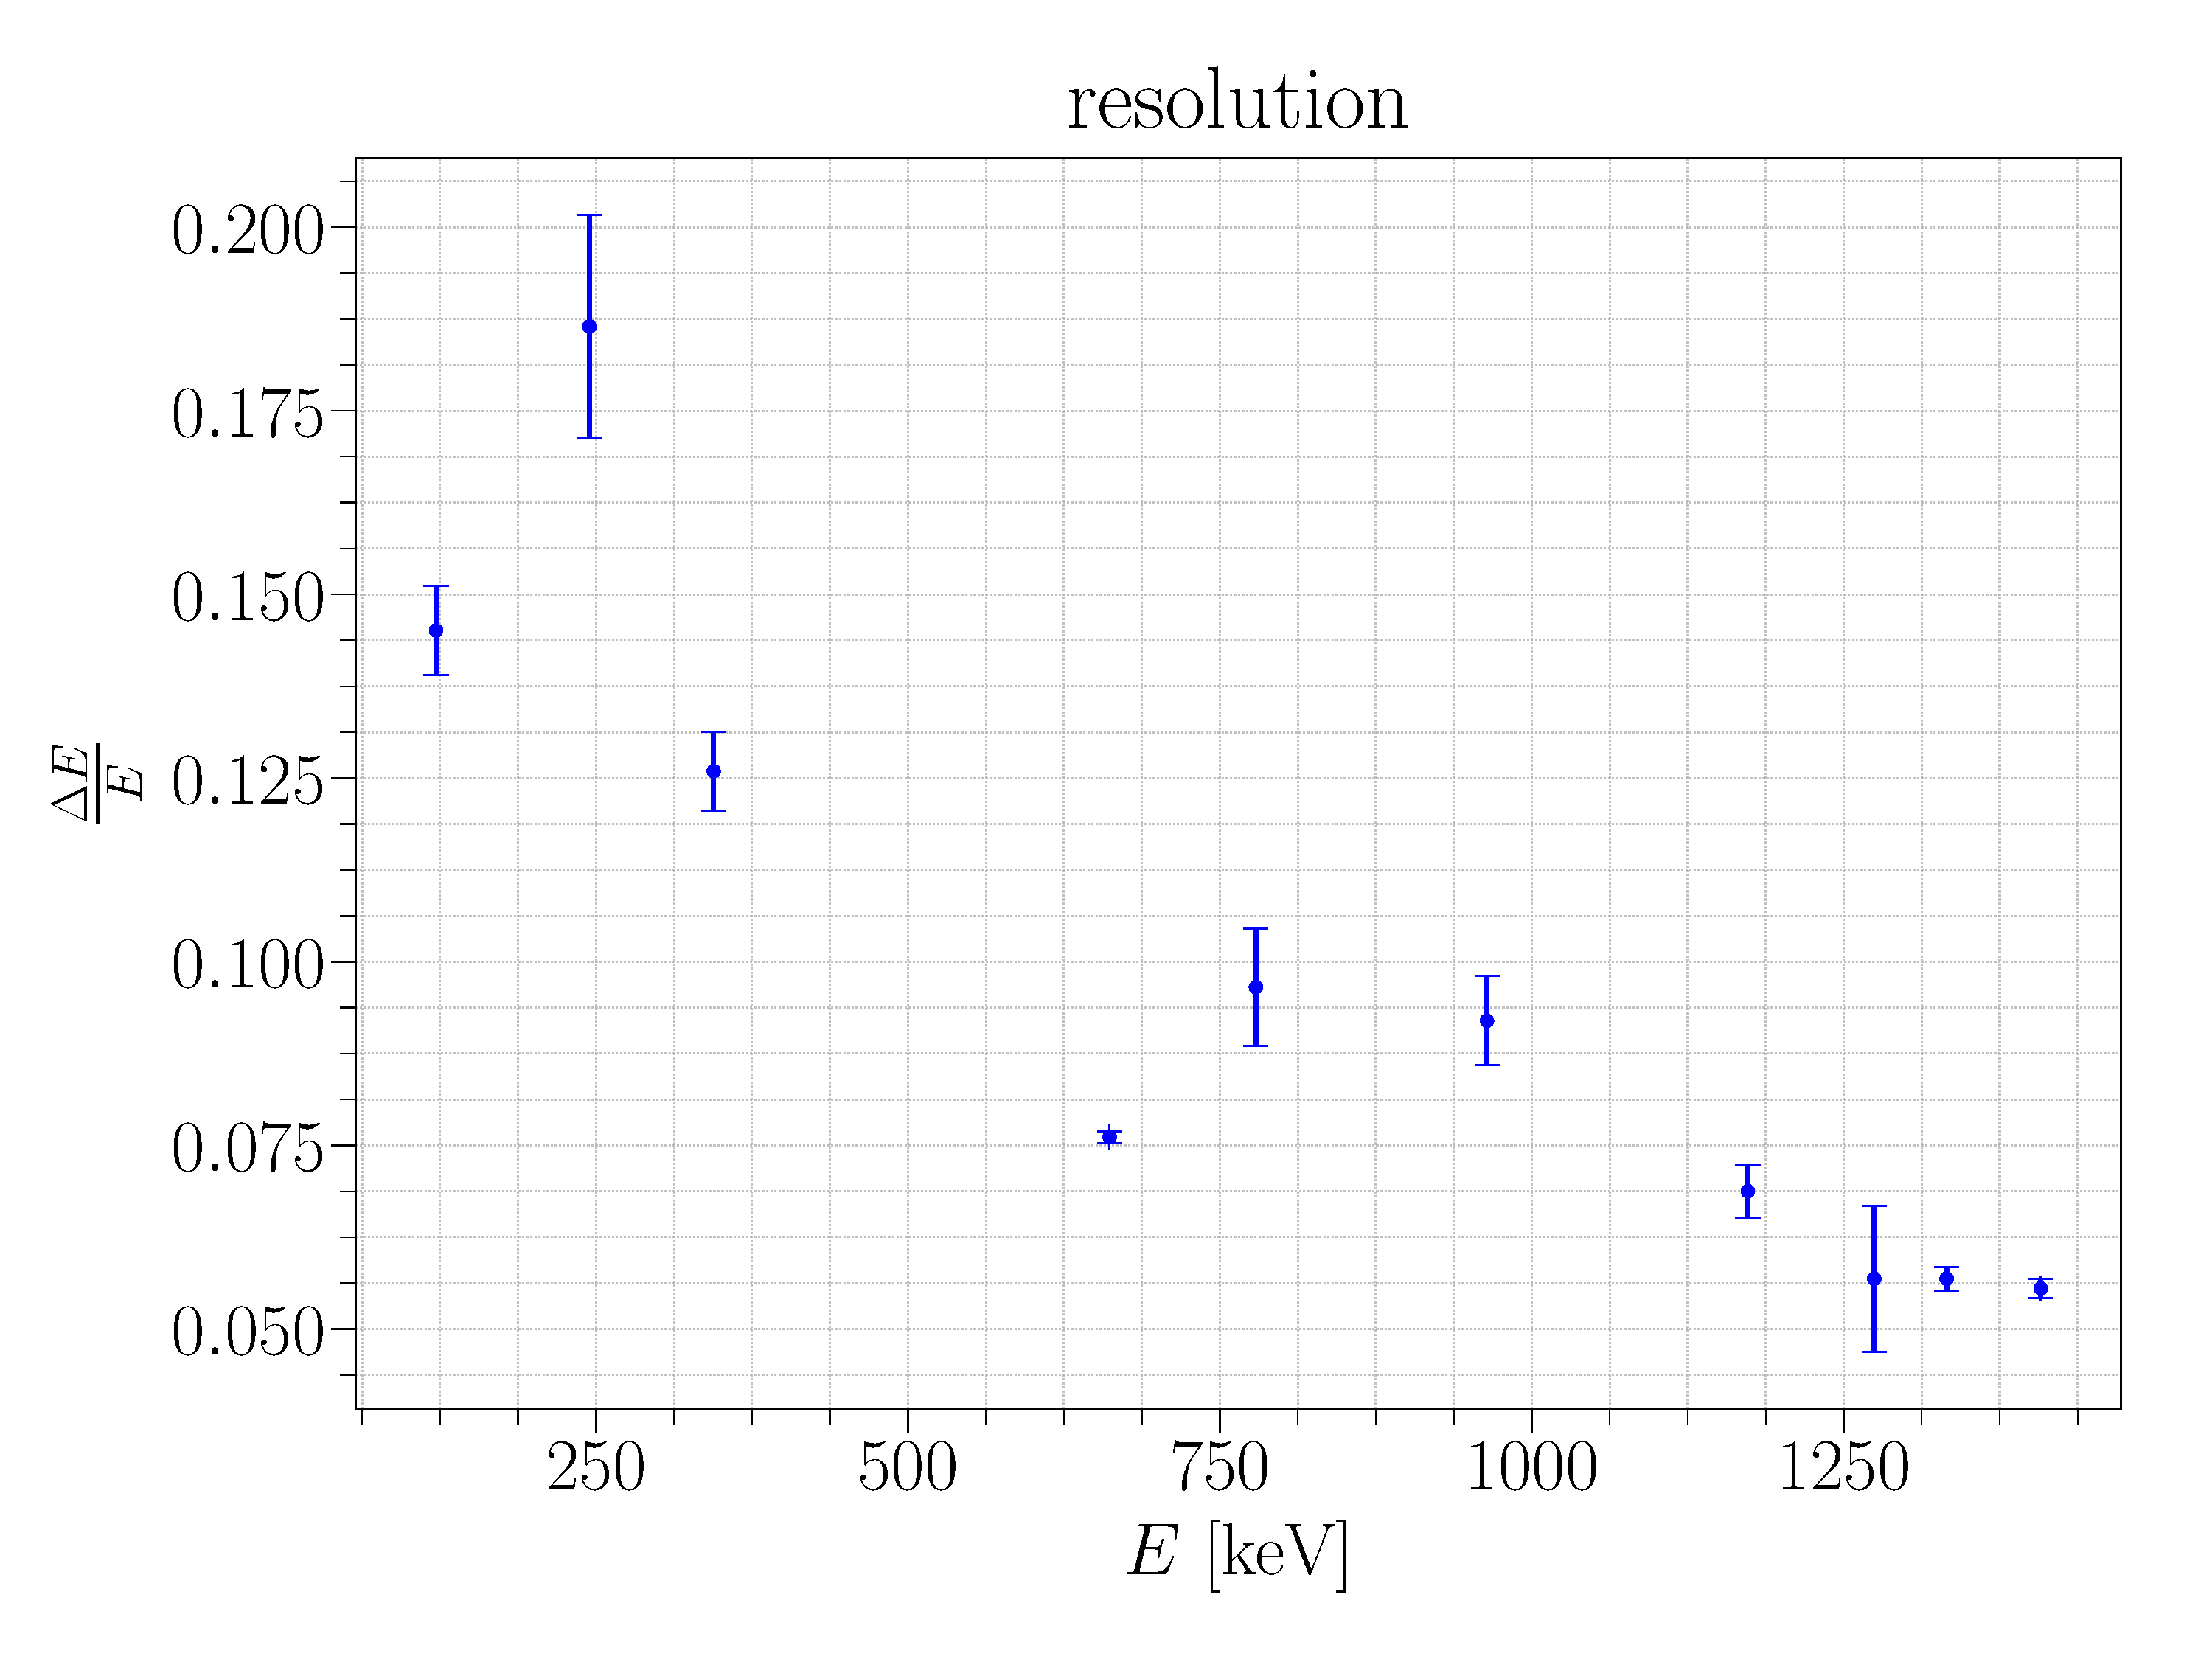
\includegraphics[scale=0.25]{../Figures/resolution.pdf}
\caption{Energy resolution vs. energy}
\label{resolution}
\end{figure}
\newpage

\begin{figure}[H]
\centering
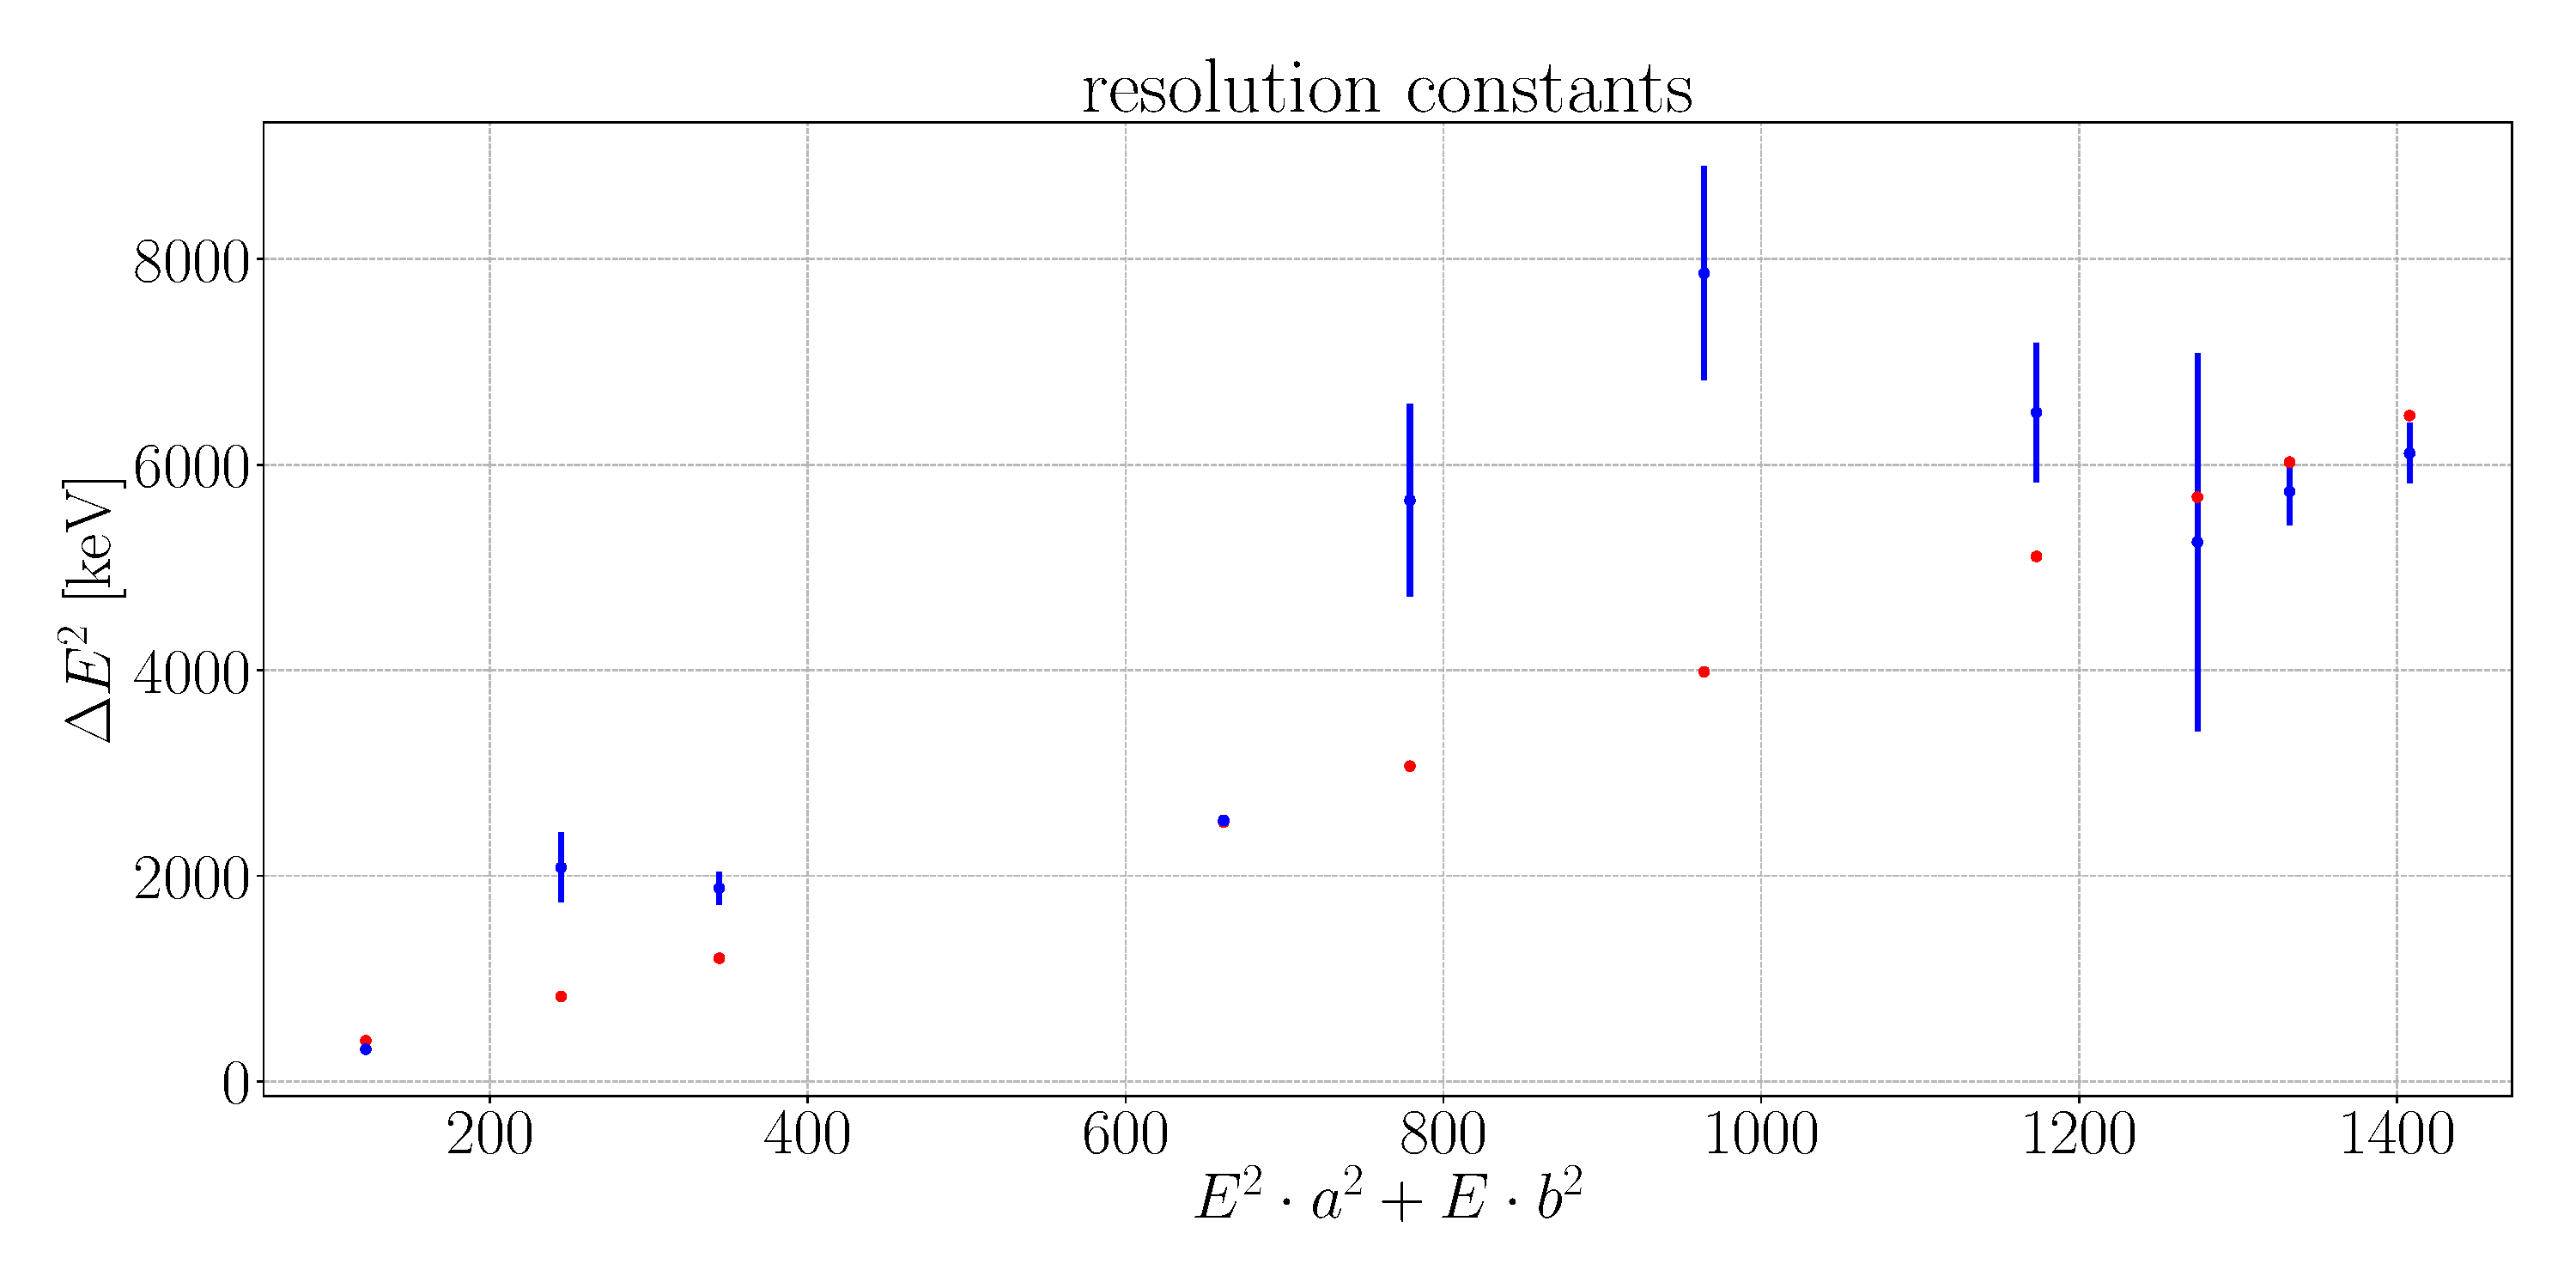
\includegraphics[scale=0.25]{../Figures/resolution constants.pdf}
\caption{Fit of $\Delta E^2 = a^2 \cdot E^2 + b^2 \cdot E$ to obtain constants in resolution}
\label{resolutionFit}
\end{figure}


\subsubsection{Efficiency}

We can compute the detector efficiency $\varepsilon$ according to 
\begin{equation}
	m = \frac{A \cdot I_\gamma}{4 \pi r_0^2} \cdot \varepsilon \cdot F_D
\end{equation}
using the counts $m$ within the FWHM of each peak. Unfortunately we can not see any functional dependence of $\varepsilon$ on the energy. Some values obtained from the Eu spectrum have large errors and lie much above the others or even above 1, but the efficiency remains nonlinear even if we exclude those. Because of this we could not get proper results for the differential cross-section in the following experiment. Our best guess for the detector efficiency is the weighted mean value of $\varepsilon = 0.25 \pm 0.02$.


\begin{figure}[H]
	\centering
	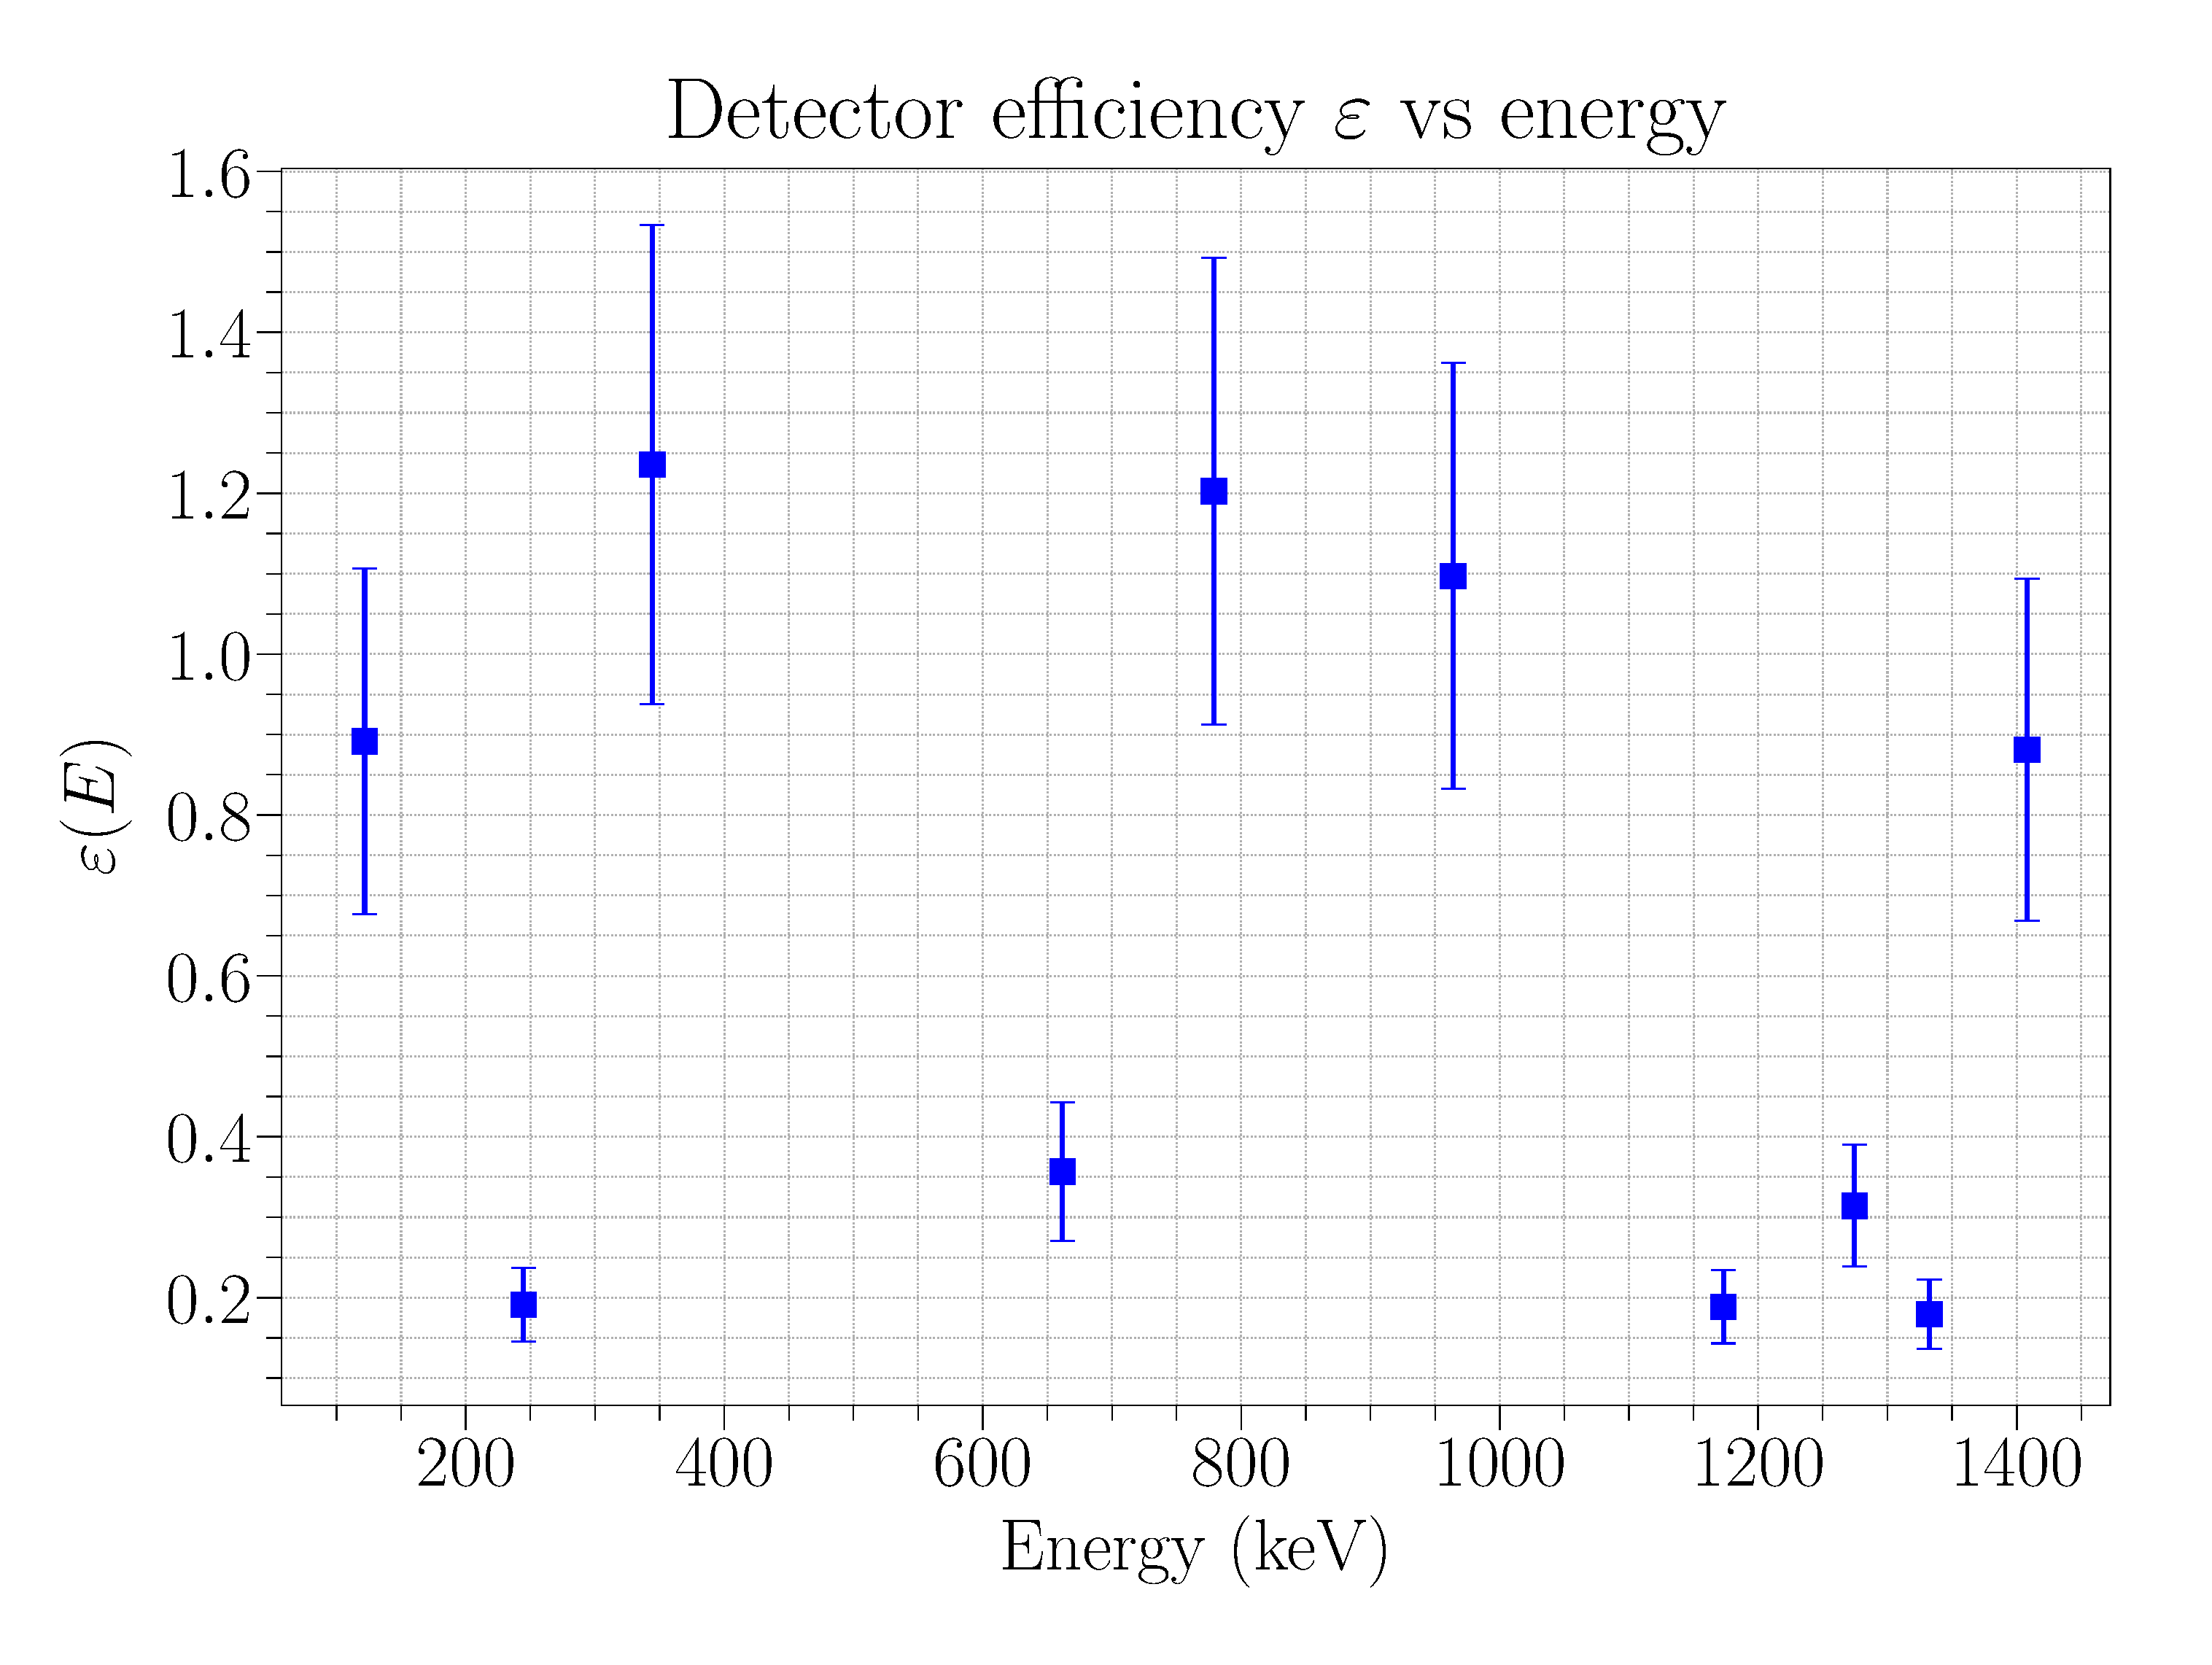
\includegraphics[scale=0.3]{../Figures/Efficiency.eps}
	\caption{Detector efficiency vs energy. The leftmost and the 3 values around 1200 keV result from Cs,Co and Na spectra, the rest belongs to Eu.}
	\label{efficiency}
\end{figure}

\subsubsection{Mass of the electron}
We can obtain the mass of the electron out of the annihilation peak in the Na spectrum, which we excluded from the calibration before. It's energy is equivalent to the electron mass. 
Using our calibration we obtain $m_e = (8.97 \pm 0.13) \times 10^{-31}$kg which has a deviation from the theory value $m_e = (9.109 \pm 0.13) \times 10^{-31}$kg of $1.07 \, \sigma$.

\begin{figure}[H]
	\centering
	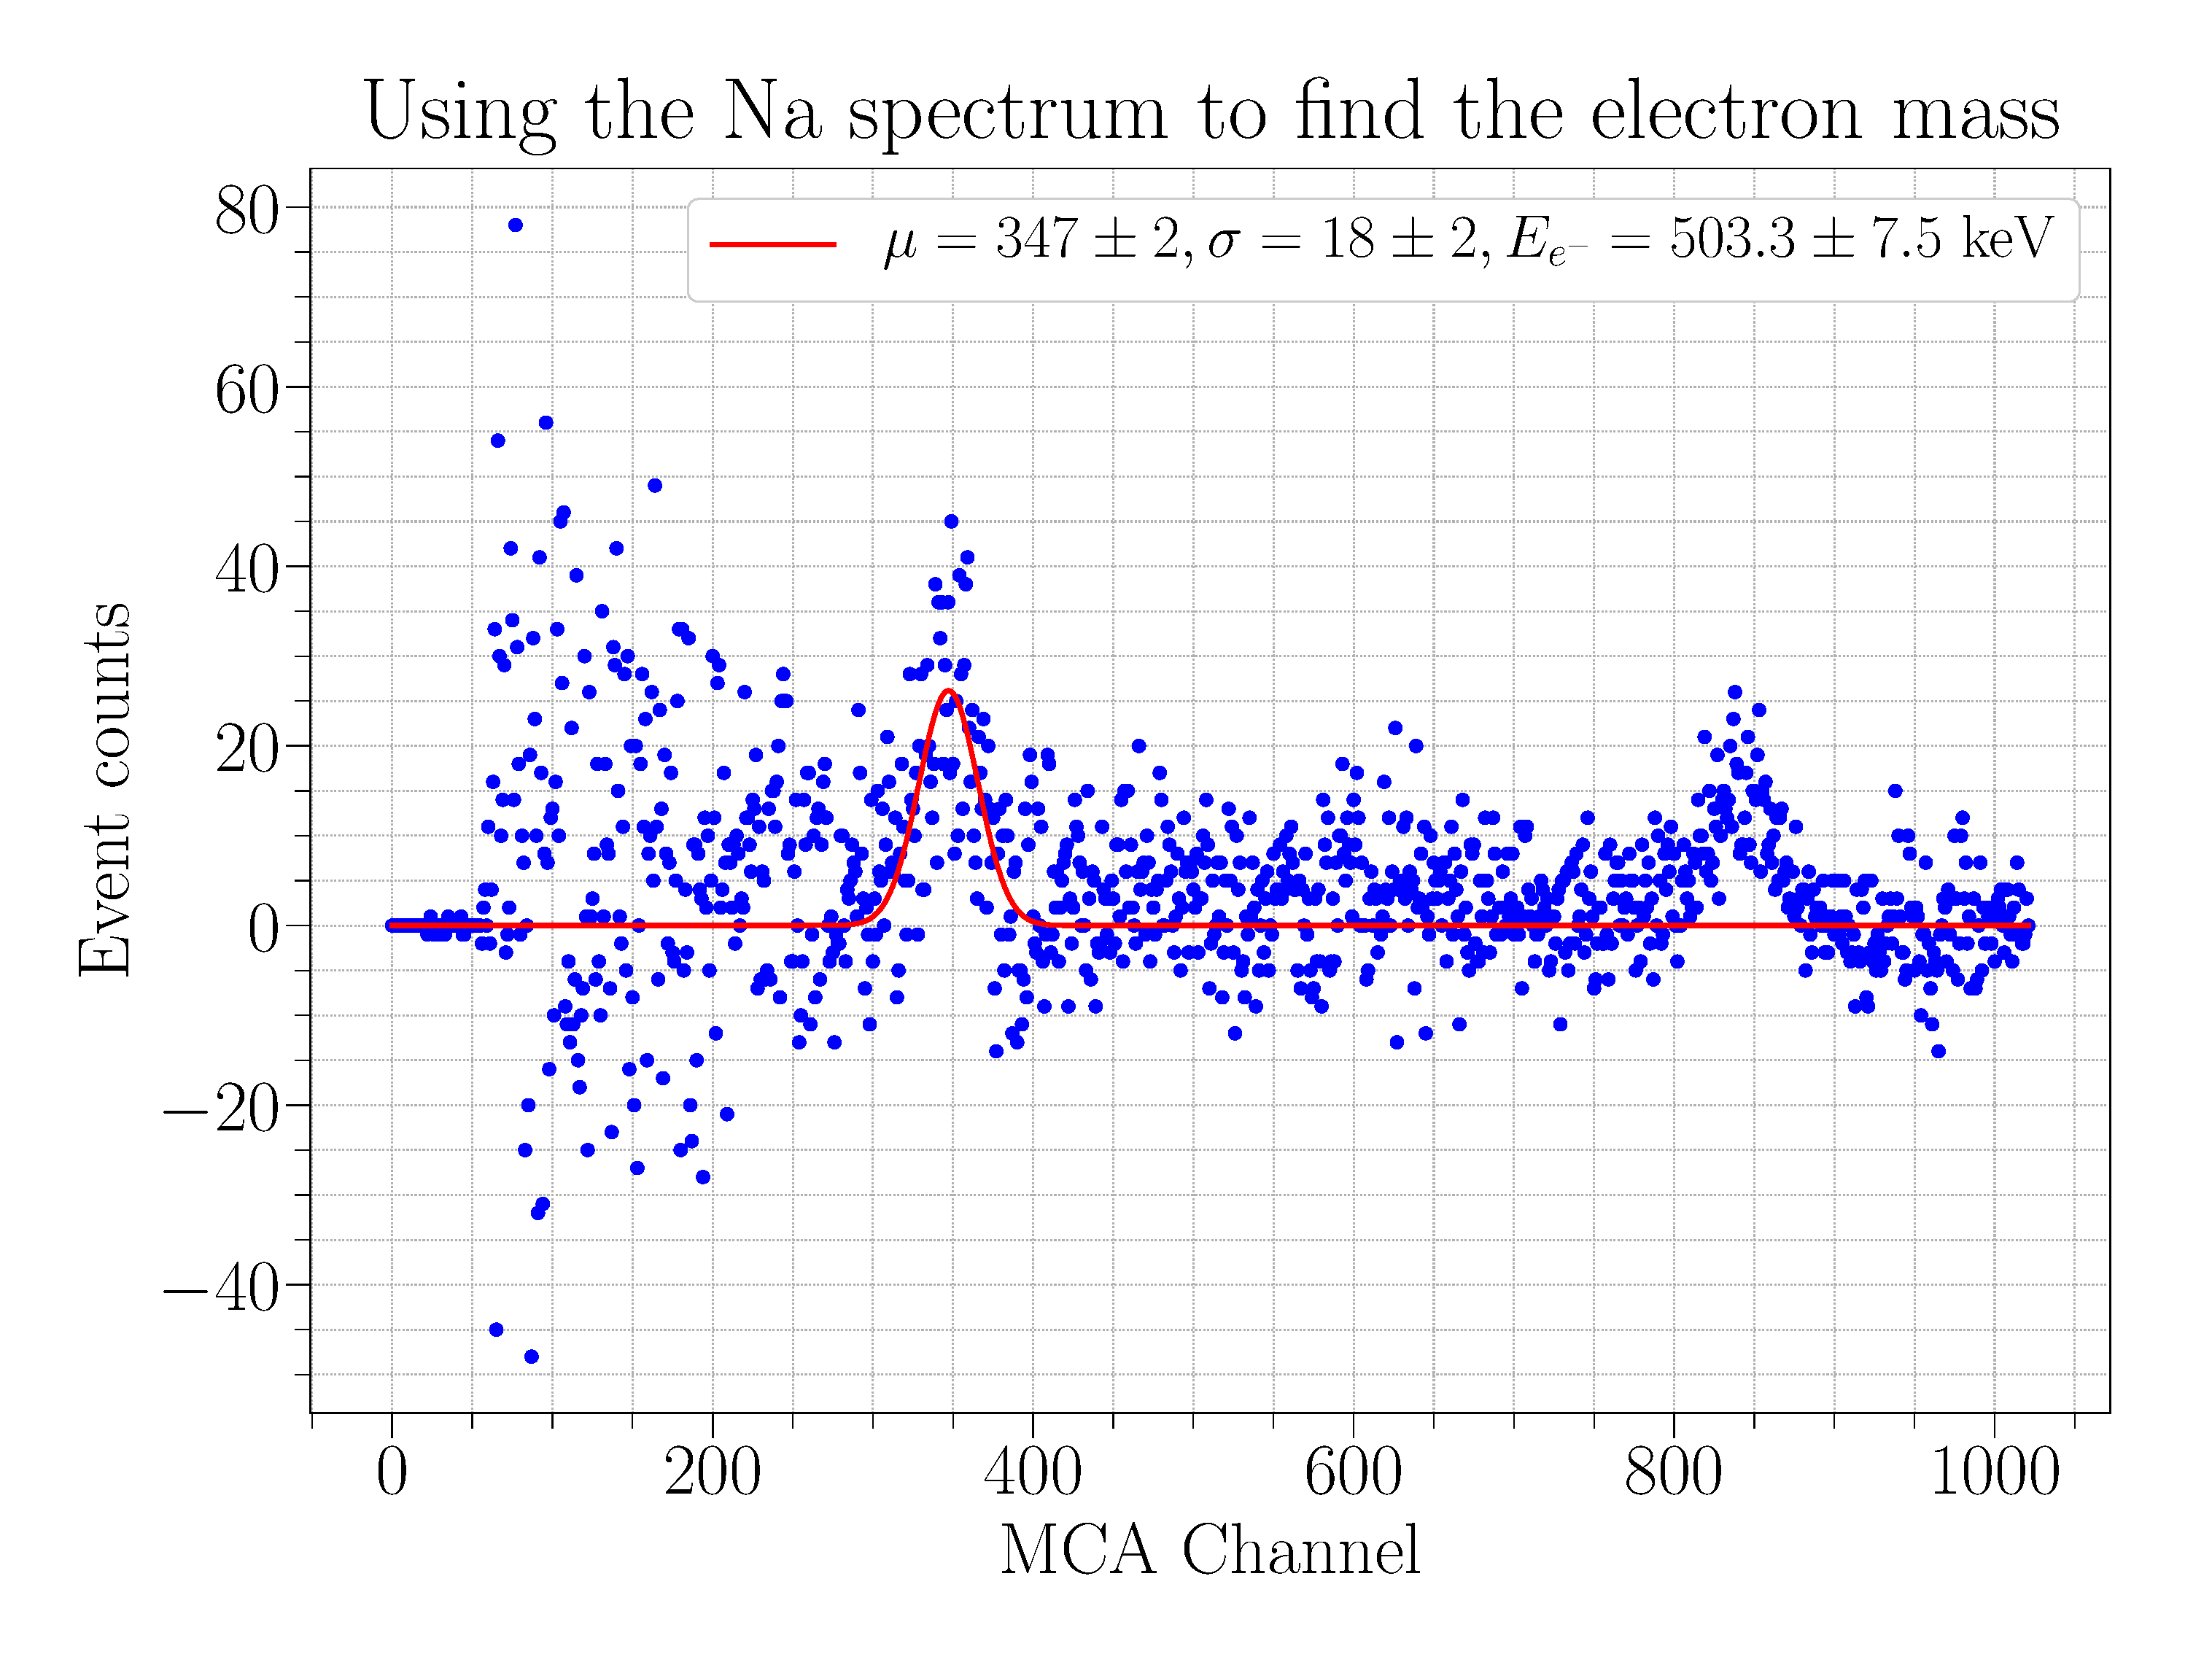
\includegraphics[scale=0.25]{../Figures/Na_me.eps}
	\caption{Fit to the annihilation peak in the Na spectrum, giving the energy of an electron.}
	\label{efficiency}
\end{figure}

\clearpage
\section{Compton scattering}

\subsection{Theory}
The energy of a photon with incoming energy $E_\gamma$, after compton scattering at angle $\theta$, is given by: 
\begin{equation}
	E_\gamma^\prime = E_\gamma \cdot \frac{1}{1+a(1-\cos\theta)} 
\end{equation}
where $a = \frac{E_\gamma}{m_e c^2}$.

The differential cross-section for such an event is given by the Klein-Nishina formula:
\begin{equation}
	\frac{d\sigma}{d\Omega} = \frac{\alpha^2\lambda_e^2}{8\pi^2} \cdot\frac{1}{\rho^2} (\rho+\frac{1}{\rho}-\sin^2\theta)
\end{equation}
where $\rho=\frac{E_\gamma}{E_\gamma^\prime} = 1+a(1-\cos\theta)$ and $\lambda_e$ is the compton wavelength.

To measure the cross-section in the experiment we can use the following relation for the count rate:
\begin{equation}
	m = \frac{A \cdot I_\gamma}{4 \pi r_0^2} \cdot \eta \cdot \epsilon \cdot N_e \cdot \frac{d\sigma}{d\Omega} \cdot \frac{F_D}{r^2}
\end{equation}

\subsection{Setup}

\subsubsection{Conventional geometry}

\begin{figure}[H]
	\centering
	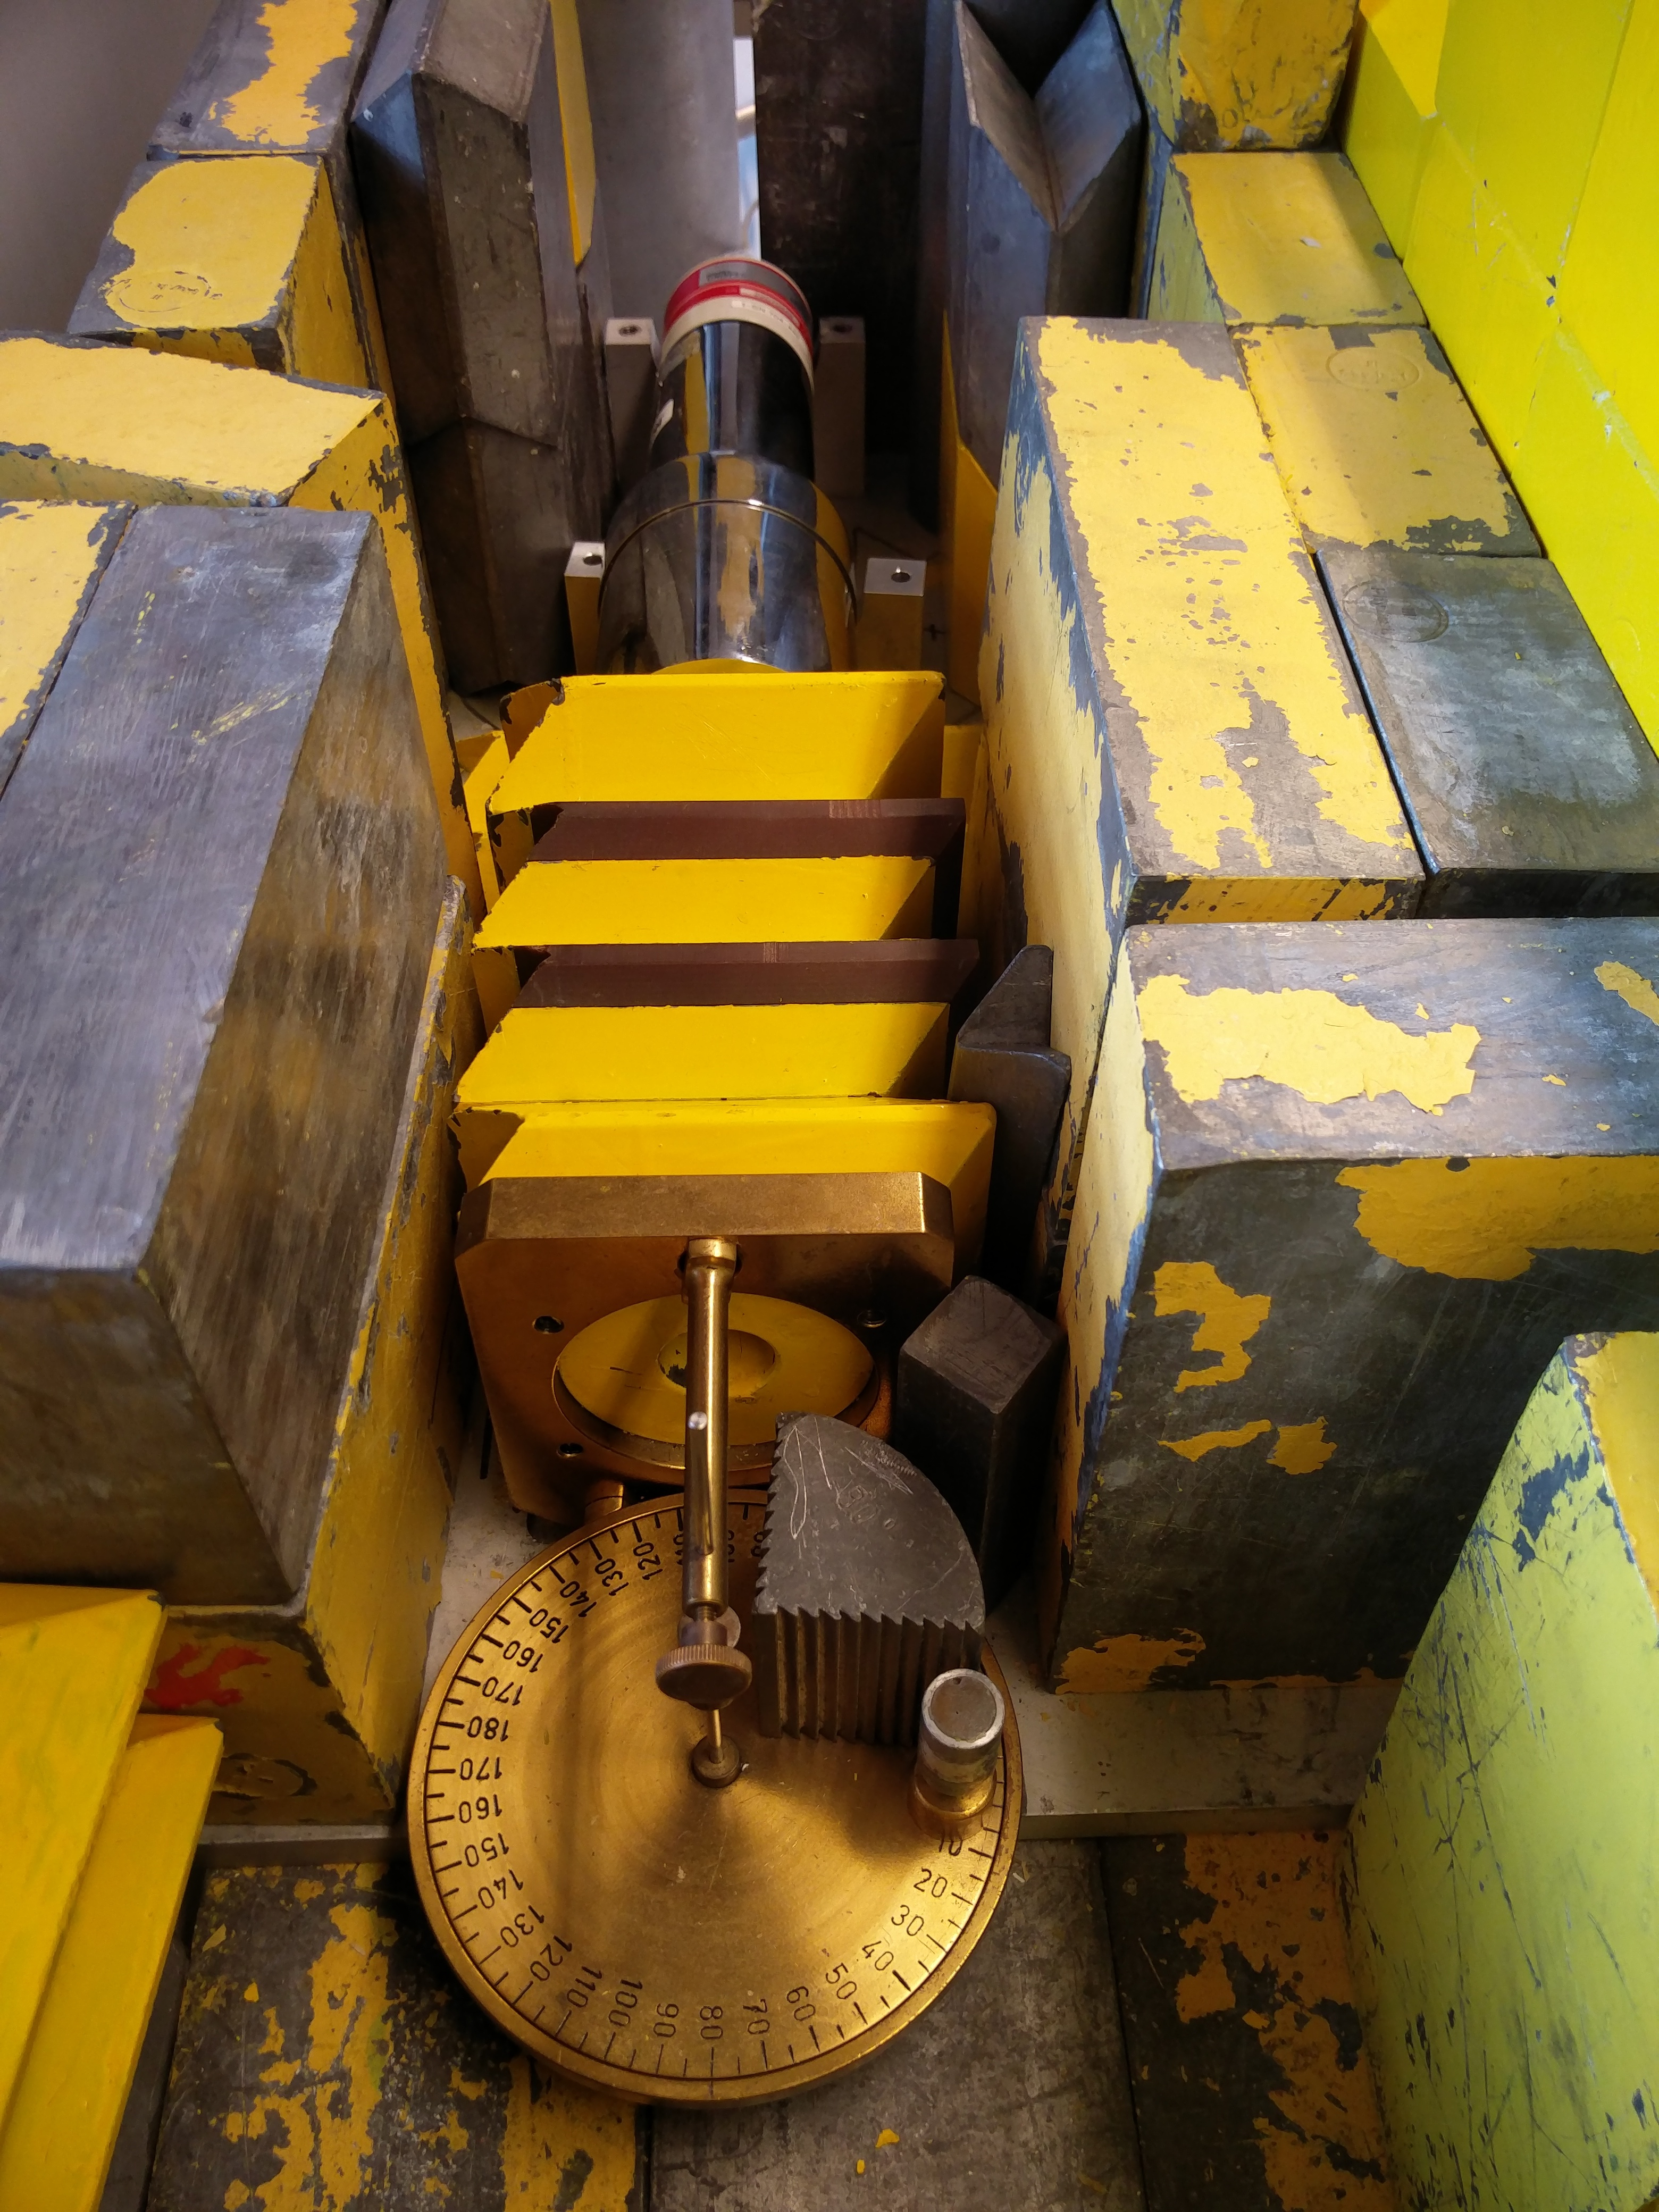
\includegraphics[scale=0.1]{../Figures/conv.jpg}
	\caption{Setup for conventional geometry}
	\label{setCalib}
\end{figure}

The source is placed on the edge of a rotating table, allowing to set different angles. In the middle of the table we place the scattering body (either a steel or an aluminum cylinder). To shield the radiation coming directly from the source from the detector, we use lead bricks shaped to match the set angle.\\
Distance from source to scattering body: $r_0 = \SI{49+-1}{mm}$\\
Distance from scattering body to detector: $r = \SI{272+-1}{mm}$\\

\subsubsection{Ring geometry}

\begin{figure}[H]
	\centering
	\includegraphics[scale=0.1]{../Figures/ring.jpg}
	\caption{Setup for ring geometry}
	\label{setCalib}
\end{figure}

For the ring geometry setup the source is aligned with the detector, but shielded of it by a lead cylinder in the middle. The scattering body is an aluminum ring placed around the lead cylinder. Therefore the whole experiment is axially symmetric.

\begin{table}[H]
	\renewcommand{\arraystretch}{1.5}
	\centering
	\begin{tabular}{|c|c|c|c|c|}
		\hline
		ring size & outer diameter $d_o$ & inner diameter $d_i$ & mean diameter $d$ & width\\
		\hline
		small & \SI{149+-1}{mm} & \SI{121+-1}{mm} & \SI{149+-1}{mm} & \multirow{3}{*}{\SI{14+-1}{mm}} \\
		\cline{1-4}
		medium & \SI{199+-1}{mm} & \SI{171+-1}{mm} & \SI{149+-1}{mm} & \\
		\cline{1-4}
		large & \SI{250+-1}{mm} & \SI{221+-1}{mm} & \SI{149+-1}{mm} & \\
		\hline
	\end{tabular}
	\caption{Compilation of measured parameters of the rings. }
	\label{tab:rings }
\end{table}

The detector was not shielded by a collimator as in the conventional geometry experiments, so we measured its size to be $d = 8.1 \pm 0.1$cm, $F_D = (51.5\pm1.3)\si{\centi\meter\squared}$. We fixed the distance between detector and ring, and measured it to be $L_d = 23.43 \pm 0.05$cm, via averaging multiple measurements on both sides.

As we needed to perform measurements for 5 different angles up to and including 50 degrees, we computed the in plane distances (along the symmetry axis) between source and ring using the geometric relation
\begin{equation}
	L_S = \frac{d}{2} \cdot \tan{\left( \pi - \arctan{\left( 2 \cdot \frac{L_D}{d} \right)} \right)}
\end{equation}
After setting the distances, we calculated the actually set angles, which may differ from the expected ones due to errors in the length measurement, which were fairly high as it was difficult to measure using the broken measurement tape in the air. We therefore used 1 cm as the error for this part. For that we used the inverse relation
\begin{equation}
	\theta = \pi - \arctan{\left( 2 \cdot \frac{L_S}{d} \right)} - \arctan{\left( 2 \cdot \frac{L_D}{d} \right)}
\end{equation}
We can then compute the diagonal distances to the ring $r, r_0$ via simple pythagorean relations. The results of this procedure are combined in \cref{tab:ringsetup}. As one can see we chose the lengths and angles such that we could just switch the ring for the first 3 angles, and only had to reset the distance to the source for the two smallest ones.

\begin{table}[H]
	\renewcommand{\arraystretch}{1}
	\centering
	\Large
	\begin{adjustbox}{width=\textwidth}
		\begin{tabular}{c|ccccc}
			\hline
			Ring used & large & medium & small & small & small \\
			\hline
			required $\theta$ & $50^\circ$ & $40^\circ$ & $30^\circ$ & $24^\circ$ & $19^\circ$ \\
			\hline
			required $L_S$ (cm) & $27.3 \pm 0.2$ & $27.7 \pm 0.2$ & $27.2 \pm 0.3$ & $48.5 \pm 0.8$ & $132 \pm 5$ \\
			\hline
			set $L_S$ (cm) & $27 \pm 1$ & $28 \pm 1$ & $27 \pm 1$ & $48 \pm 1$ & $132 \pm 1$ \\
			\hline
			set $\theta$ & $50.2 \pm 0.8$ & $39.8 \pm 0.6$ & $30.1 \pm 0.5$ & $24.1 \pm 0.2$ & $19.0 \pm 0.1$ \\
			\hline
			$r$ (cm) & $26.22 \pm 0.05$ & $25.19 \pm 0.05$ & $24.38 \pm 0.05$ & $24.38 \pm 0.05$ & $24.38 \pm 0.05$ \\
			\hline
			$r_0$ (cm) & $29.5 \pm 0.9$ & $29.5 \pm 0.9$ & $28 \pm 1$ & $48 \pm 1$ & $132 \pm 1$ \\
			\hline
		\end{tabular}
	\end{adjustbox}
	\caption{Compilation of measurements for the ring setup. }
	\label{tab:ringsetup}
\end{table}
 

\subsection{Analysis}

\subsubsection{Finding scattered photons}

The results of the peak energies in dependence of the scattering angle are shown in \cref{Ephi}. Here blue datapoints represent data from the ring setup, orange and green points are results of the conventional setup using aluminum and metal scattering cylinders, respectively. We see no significant difference between the material of the scattering body. Comparing the results for a scattering angle of $\theta = 50 ^\circ$ we see that the peak from the ring geometry has a slightly higher energy than the ones from the conventional one. The data matches the curve expected by theory fairly well, except for very small angles, which is shown in red.

\begin{figure}[H]
\centering
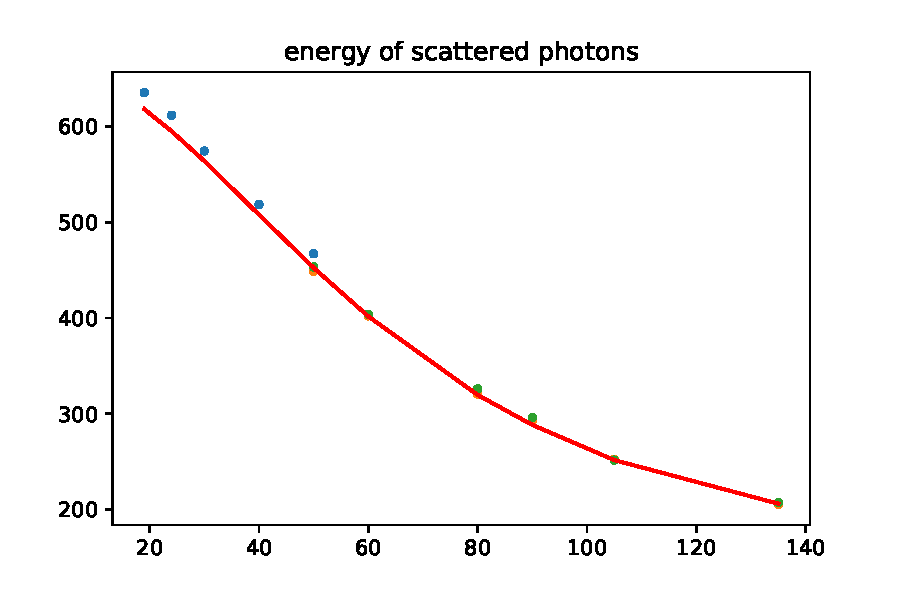
\includegraphics[scale=1]{../Figures/E_Phi.pdf}
\caption{Energy of scattered photons vs. scattering angle}
\label{Ephi}
\end{figure}



\clearpage
\section{Appendix}

\subsection{Raw data of gamma spectroscopy experiment}

\begin{figure}[H]
	\centering
	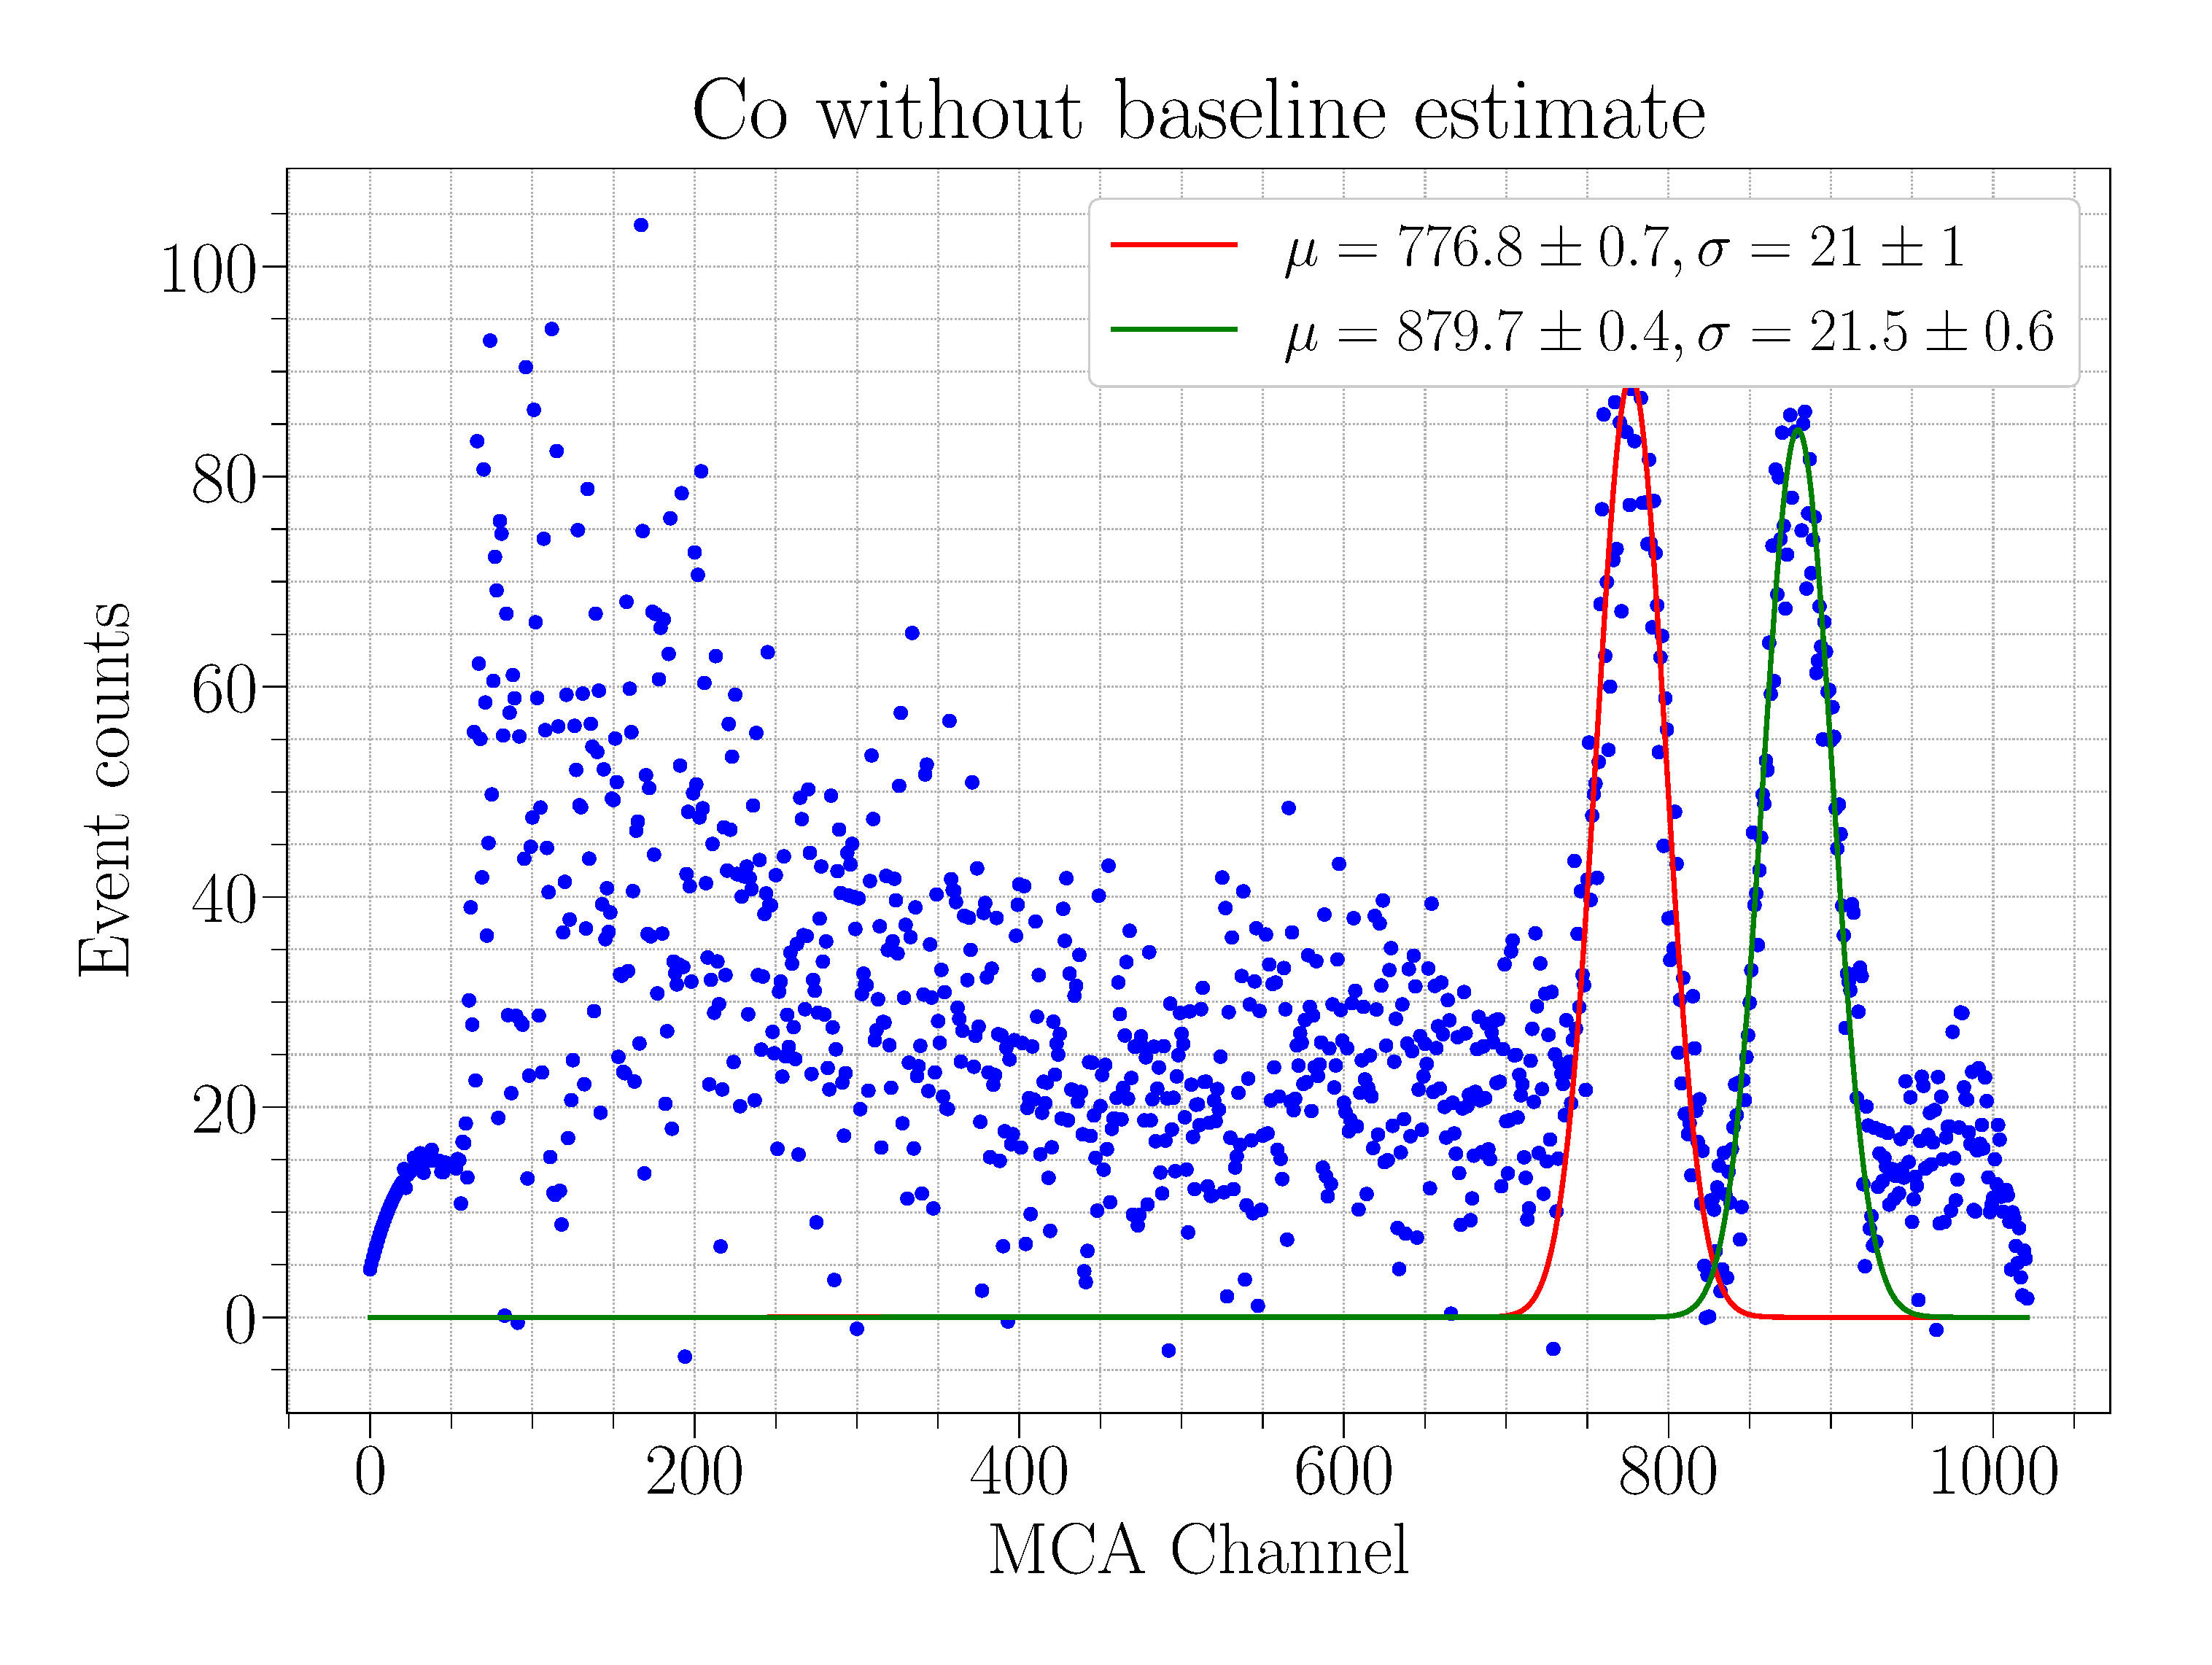
\includegraphics[scale=0.25]{../Figures/Co_nobaseline.eps}
	\caption{}
	\label{Eu_raw}
\end{figure}

\begin{figure}[H]
	\centering
	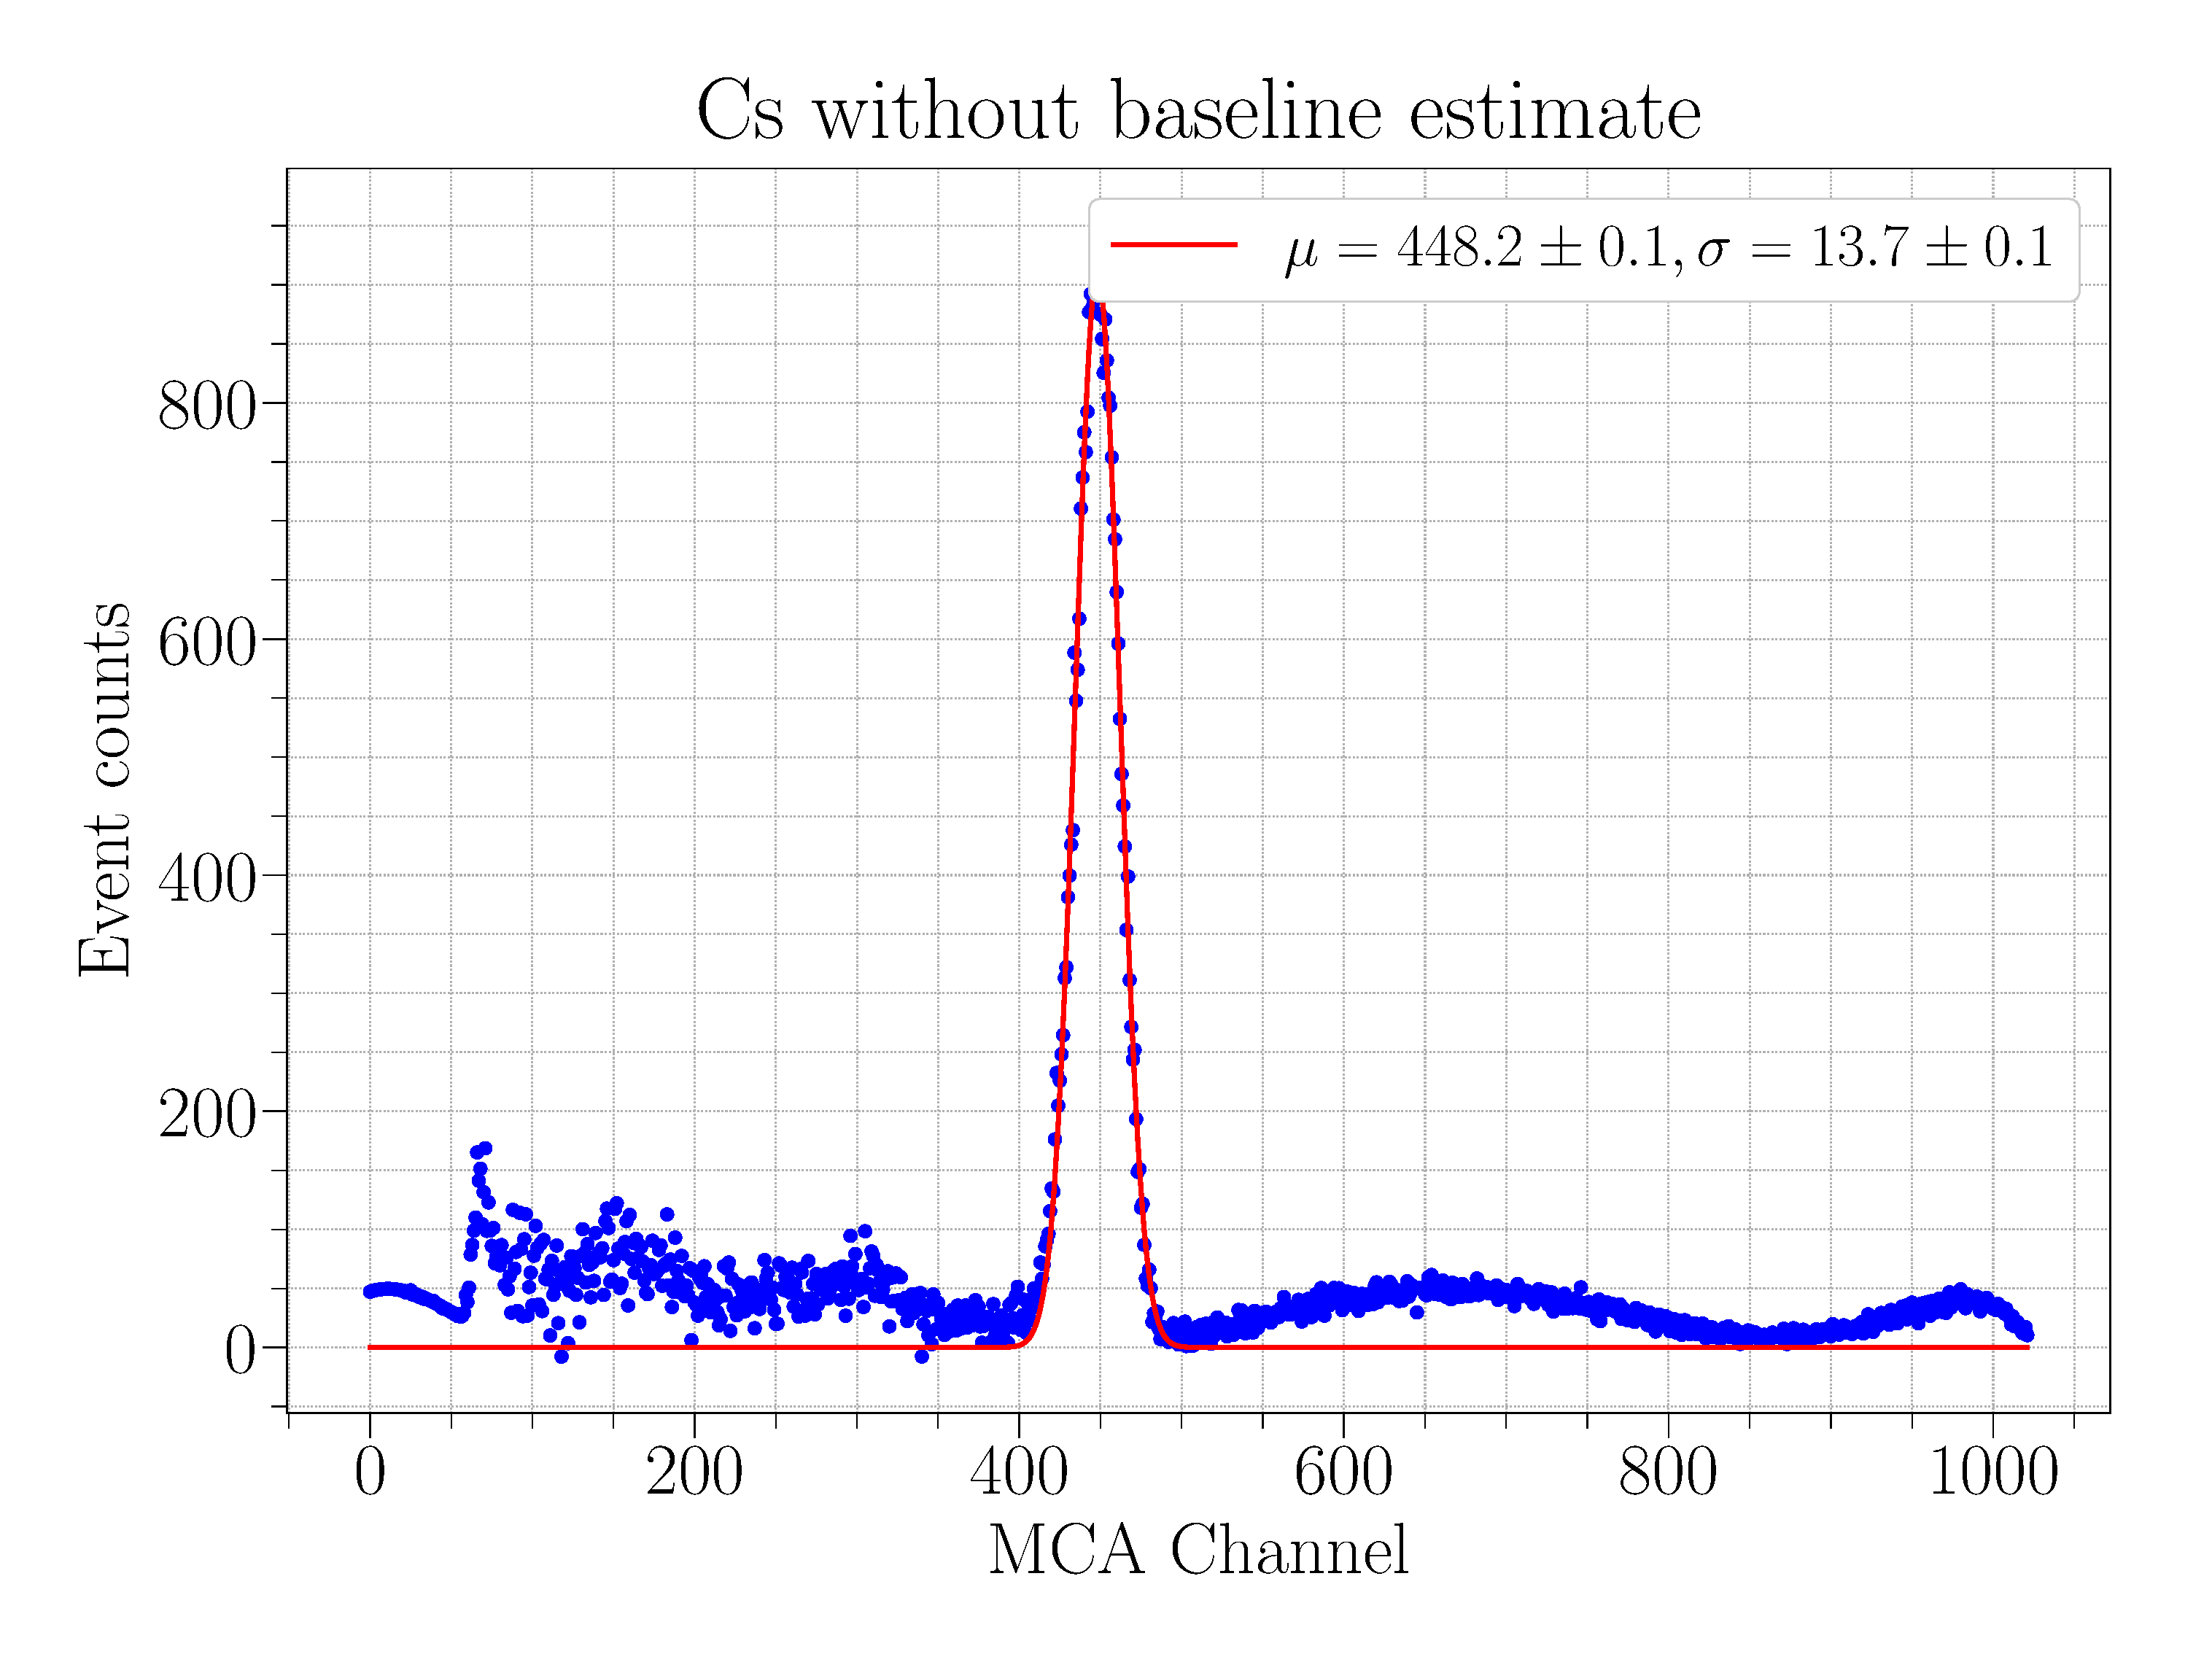
\includegraphics[scale=0.25]{../Figures/Cs_nobaseline.eps}
	\caption{}
	\label{Eu_raw}
\end{figure}

\begin{figure}[H]
	\centering
	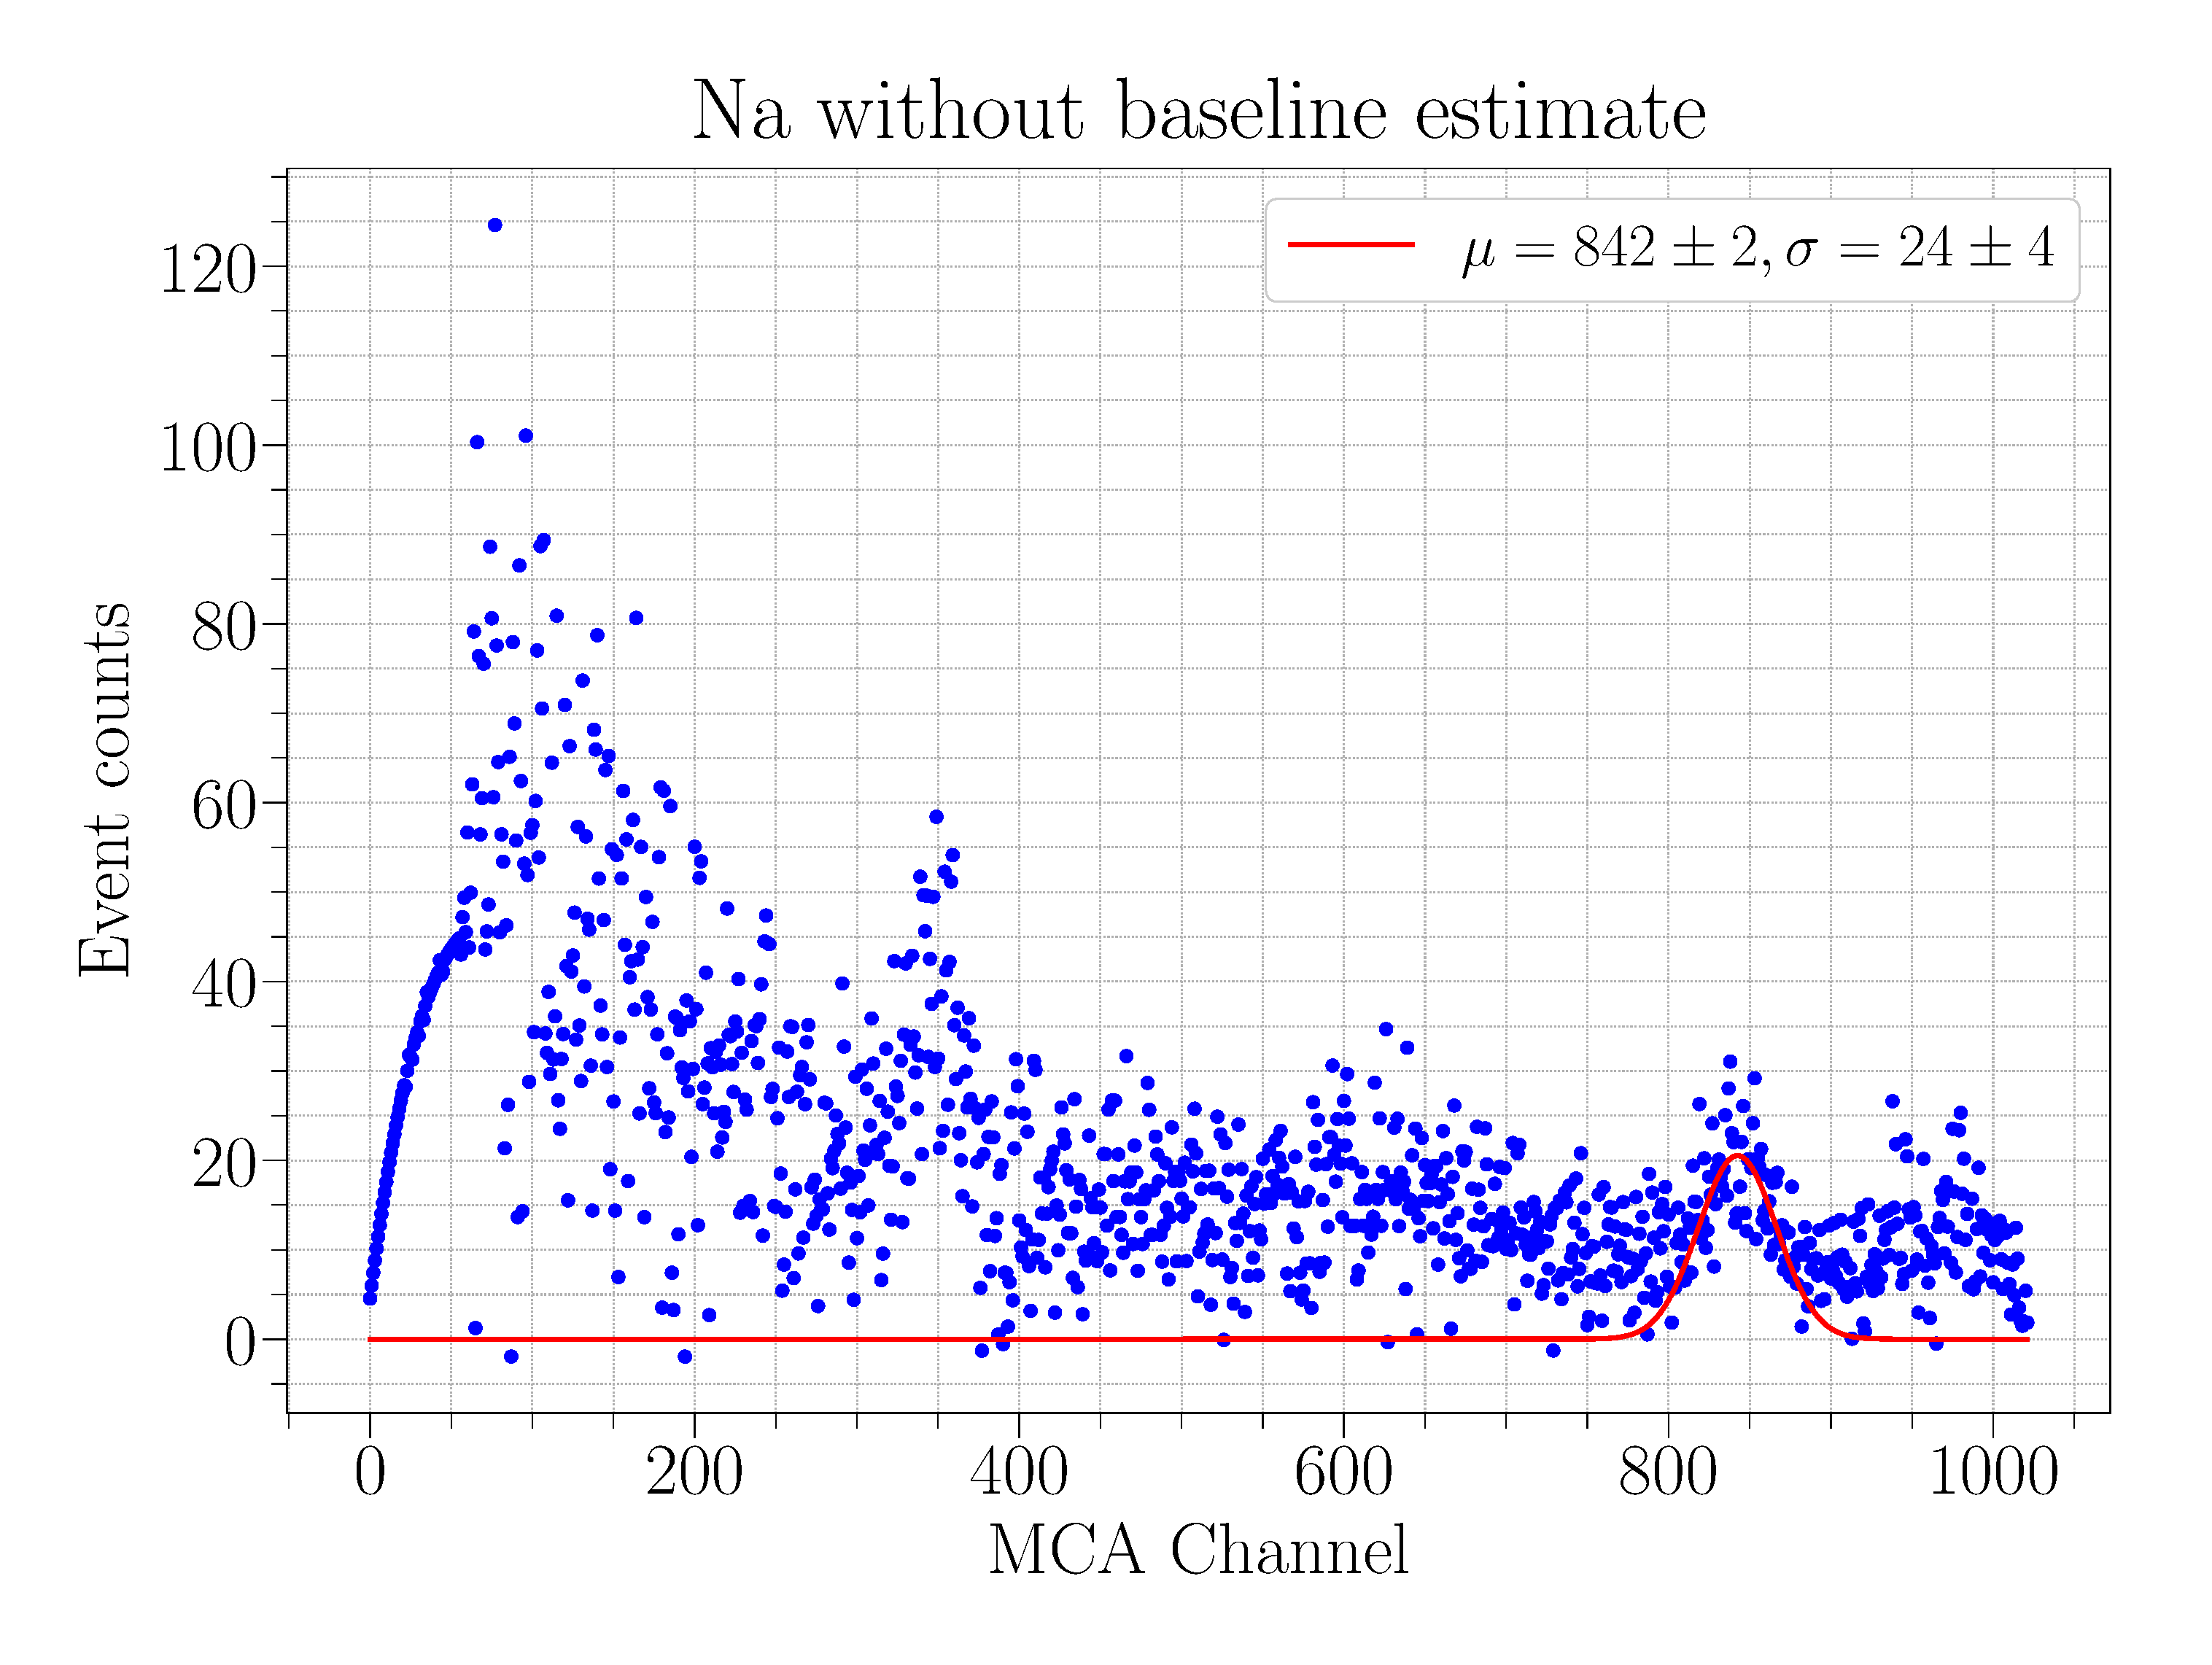
\includegraphics[scale=0.25]{../Figures/Na_nobaseline.eps}
	\caption{}
	\label{Eu_raw}
\end{figure}

\subsection{Raw data of Compton scattering experiments}

\foreach \angle in {50,60,80,90,105,135}{
	\begin{figure}[H]
		\centering
		\includegraphics[scale=0.25]{../Figures/\angle_Conv_Fe.pdf} 
		\caption{Raw data of conventional setup with metal as scattering cylinder for an angle of $\theta=\,$\angle$^\circ$}
		\label{fig:}
	\end{figure}
}

\foreach \angle in {50,60,80,90,105,135}{
	\begin{figure}[H]
		\centering
		\includegraphics[scale=0.25]{../Figures/\angle_Conv_Al.pdf} 
		\caption{Raw data of conventional setup with aluminum as scattering cylinder for an angle of $\theta=\,$\angle$^\circ$}
		\label{fig:}
	\end{figure}
}

\foreach \angle in {19,24,30,40,50}{
	\begin{figure}[H]
		\centering
		\includegraphics[scale=0.25]{../Figures/\angle_Ring.pdf} 
		\caption{Raw data of ring setup for an angle of $\theta=\,$\angle$^\circ$}
		\label{fig:}
	\end{figure}
}



\end{document}